
\documentclass{article}

% Formatting
\usepackage[utf8]{inputenc}
\usepackage[margin=1in]{geometry}
\usepackage[titletoc,title]{appendix}

\usepackage{comment}
\usepackage{soul}
\usepackage{xcolor}
% Images
% https://www.overleaf.com/learn/latex/Inserting_Images
% https://en.wikibooks.org/wiki/LaTeX/Floats,_Figures_and_Captions
\usepackage{graphicx,float}

% Subfigures
\usepackage{subfigure}

% References
% https://www.overleaf.com/learn/latex/Bibliography_management_in_LaTeX
% https://en.wikibooks.org/wiki/LaTeX/Bibliography_Management
\usepackage{biblatex}
\addbibresource{report/references.bib}

% Math & algorithms
% >>>>>>>>>>>>>>>>>>>>>>>>>>>>>>>>>>>>>> %
%           MATHS                        %
% >>>>>>>>>>>>>>>>>>>>>>>>>>>>>>>>>>>>>> % 
% https://www.overleaf.com/learn/latex/Mathematical_expressions
% https://en.wikibooks.org/wiki/LaTeX/Mathematics
\usepackage{amsmath,amsfonts,amssymb,mathtools, bbold, bbm}

% Algorithms
% https://www.overleaf.com/learn/latex/algorithms
% https://en.wikibooks.org/wiki/LaTeX/Algorithms
%\usepackage[ruled,vlined]{algorithm2e}
%\usepackage{algorithmic}
\usepackage[ruled,vlined]{algorithm2e}
% Colored comments
\newcommand\mycommfont[1]{\ttfamily\textcolor{blue}{#1}}
\SetCommentSty{mycommfont}


% Make mathbb nice (e.g. set of real number R: \mathbb R)
% https://tex.stackexchange.com/questions/58098/what-are-all-the-font-styles-i-can-use-in-math-mode
\AtBeginDocument{
  \DeclareSymbolFont{AMSb}{U}{msb}{m}{n}
  \DeclareSymbolFontAlphabet{\mathbb}{AMSb}
}

% Double struck zero matrix
% https://tex.stackexchange.com/a/399950/217578
\DeclareMathAlphabet{\mymathbb}{U}{BOONDOX-ds}{m}{n}

% Custom commands & operators: vectors, matrice operations, expectations, variance, ...
\newcommand{\vect}[1]{\boldsymbol{\mathbf{#1}}}
\newcommand{\R}{\mathbb R}
\newcommand{\norm}[1]{\Vert #1 \Vert}
\DeclareMathOperator{\trace}{Tr}
\DeclareMathOperator{\E}{\mathbb{E}}
\DeclareMathOperator{\Var}{\mathbb{V}ar}

\DeclareMathOperator*{\argmin}{arg\,min}

% Double-bar Identity matrix: with or without size argument
% https://tex.stackexchange.com/questions/409760/detect-no-argument-in-newcommand
\makeatletter
\def\Id{\@ifnextchar[\Id@command{\mathbb I}}
\def\Id@command[#1]{\mathbb I_{#1}}
\makeatother

% Theorem, lemmas, corollaries, proofs, ...
\usepackage{amsthm} % proof
%\newtheorem{theorem}{Theorem}[section]
%\newtheorem{corollary}{Corollary}[theorem]
%\newtheorem{lemma}[theorem]{Lemma}
%\newtheorem{proposition}[theorem]{Proposition}
%\newtheorem*{remark}{Remark}
%\newtheorem{observation}[theorem]{Observation}
% The setup_math.tex file might be included in the slides, where the beamer package already defines theorems & co, so check if they're already defined before adding them
% https://tex.stackexchange.com/questions/41496/how-to-define-an-environment-only-if-it-is-not-defined-yet-using-etoolbox
\ifcsmacro{definition}{}{
  \let\endtheorem\undefined%
  \newtheorem{definition}{Definition}[section]
}
\ifcsmacro{theorem}{}{
  \let\endtheorem\undefined%
  \newtheorem{theorem}{Theorem}[section]
}
\ifcsmacro{corollary}{}{
  \let\endcorollary\undefined%
  \newtheorem{corollary}{Corollary}[theorem]
}
\ifcsmacro{lemma}{}{
  \let\endlemma\undefined%
  \newtheorem{lemma}[theorem]{Lemma}
}
\ifcsmacro{proposition}{}{
  \let\endproposition\undefined%
  \newtheorem{proposition}[theorem]{Proposition}
}
\ifcsmacro{remark}{}{
  \let\endremark\undefined%
  \newtheorem*{remark}{Remark}
}
\ifcsmacro{observation}{}{
  \let\endobservation\undefined%
  \newtheorem{observation}[theorem]{Observation}
}


% <<<<<<<<<<<<<<<<<<<<<<<<<<<<<<<<<<<<<< %
%           MATHS                        %
% <<<<<<<<<<<<<<<<<<<<<<<<<<<<<<<<<<<<<< %

% Title content
\title{
    {\huge \textbf{Randomized Algorithms for \\Gaussian Process Regression}}\\
}
\author{Matthias Zeller}
\date{\today}


\begin{document}

\maketitle

\section{Introduction}

Gaussian process (GP) regression is a non-parametric supervised method that extends Bayesian linear regression \cite{schulz_tutorial_2018, rasmussen_gaussian_2005, liu_when_2019, deringer_gaussian_2021}.
Considering the problem of inferring an unknown function $f$ given some inputs and noisy outputs, the GP regression setting models the prior on $f$ as a GP. Based on a-priori knowledge (e.g. the smoothness of $f$), one sets the GP mean and covariance functions and performs inference in the induced function space. 
%, which is entirely determined by its mean and covariance function. Hence, one parametrizes the prior function space according to  
%Considering the problem of inferring an unknown function $f$ specifying the relationship between inputs $\vect x_i$ and outputs $y_i$, the GP regression framework models $f$ as a GP, and hence models a Gaussian probability distribution over function values\footnote{for a fixed and finite number of points at which we evaluate $f$.}. 

GP models are attractive due to their ability to approximate a wide range of functions with interpretable hyperparameters \cite{rasmussen_gaussian_2005, belyaev_exact_2014},
they provide uncertainty estimates \cite{rasmussen_gaussian_2005, seeger_gaussian_2004}
and cast hyperparameter selection as an optimization problem \cite{gorbach_model_2017, rasmussen_gaussian_2005, seeger_gaussian_2004}.
However, exact \textcolor{red}{exact????} GP inference is traditionally done with Cholesky decomposition and requires $\mathcal O(n^2)$ memory and $\mathcal O(n^3)$ time complexity, with $n$ the number of samples in the training set, therefore suffering from scalability to large datasets. The GPyTorch framework \cite{gardner_gpytorch_2021} proposes a more efficient approach for GP inference that i) achieves sub-cubic time complexity for exact\footnote{Exact refers to the fact that one can choose parameters of the algorithms to reach machine precision, although those parameters may be unknown apriori.} inference under some suitable conditions\footnote{In the paper, it is stated that GPyTorch reduces exact GP inference to $\mathcal O(n^2)$ time complexity, which may be true in practice depending on the dataset at hand. This is related to the data distribution and the spectrum of the kernel matrix, see the discussion in the results section.}, ii) requires the user to only provide blackbox matrix-matrix multiplication oracles with the kernel matrix and its derivative.
As a consequence the framework disentangles the model from the inference engine, greatly easing implementation for the user, specifically for complex GP models (e.g., combining different kernels or using GP approximations for large datasets). 

The core of GPyTorch is based on a combination of conjugate gradients, Lanczos quadrature and stochastic trace estimation to compute the likelihood of the model hyperparameters and its gradient. A specialized preconditioner is used to speedup CG convergence and reduce the overall complexity.

The rest of this introduction reviews GP regression and how this can be derived from Bayesian linear models. We introduce the different quantities involved and the approach for estimating unknown parameters. In section~\ref{sec:training}, we discuss the training of GPs for regression, the algorithms used in GPyTorch and the underlying theory. Section~\ref{sec:precond} exposes a preconditioning approach suited for some kernel matrices. The convergence is then analyzed and discussed in section~\ref{sec:convergence}. Numerical results are eventually presented in section~\ref{sec:numexp}.
\textcolor{red}{Generally, this introduction is good.}

%Gaussian Processes are a generalization of Gaussian probability distributions which can be used in a supervised learning setting to perform regression (or classification). Considering the problem of inferring an unknown function $f$ specifying the relationship between inputs $\vect x_i$ and outputs $y_i$, the Gaussian Process framework consists in modeling an estimator function $f^\star$ as a Gaussian process. Exact inference requires inversion of 

%Gaussian Processes are a generalization of Gaussian probability distributions which can be used in a supervised learning setting to perform regression or classification. A Gaussian Process is a stochastic process whose any finite number of points can be characterized by a joint normal distribution. Considering the supervised problem of inferring an unknown function $f$ modeling the relationship between inputs $\vect x_i$ and outputs $y_i$, the Gaussian Process framework consists in modeling the estimator function $f^\star$ as a Gaussian process. We will note $f^\star \sim \mathcal{GP}(\mu, k)$ with $\mu : \R^d \to \R$ the mean function and $k: \R^d \times \R^d \to \R$ the covariance function. 


\subsection{Review Bayesian Linear Regression}

Given a training dataset $\mathcal D = \{(\vect x_i, y_i)\}_{i=1}^n$ and assuming there is an unknown function $f$ following the measurement model with Gaussian noise

\begin{equation} \label{eq:measurement_model}
    y_i = f(\vect x_i) + \epsilon_i, \quad \epsilon_i \sim \mathcal N(0, \sigma^2) \; ,
\end{equation}
\textcolor{red}{you have indenting everywhere after equations. Please remove them.}
%
one wishes to predict $f(\vect x^\star)$ for samples $\vect x^\star$ that were not in the training set. We focus on the Bayesian linear regression with a Gaussian prior for the weights, i.e. $f(\vect x) = \vect w^\top \vect x$, $\vect w \sim \mathcal N(\vect 0, \Sigma_0)$. One performs predictions by considering the posterior distribution $f (\vect x^\star) \mid \mathcal D$, whose density is expressed in terms of the likelihood $p(\vect y \mid X, \vect w)$ and the prior $ p(\vect w)$.

This model can be extended by introducing basis functions $\vect \phi : \R^d \to \R^D$ (independent of $\vect w$), where typically $D \gg d$. One projects the features $\vect x$ onto the feature space $\vect\phi(\R^d)$, so that the new model is $f(\vect x) = \vect w^\top \vect \phi(\vect x)$, which remains linear in the feature space. It turns out one can express the posterior distribution solely in terms of inner products of the form

\begin{equation} \label{eq:kernel_trick}
    \vect\phi(\vect x)^\top \Sigma_0 \vect\phi(\vect x') \;,
\end{equation}

this is often referred to the \emph{kernel trick} (see \cite{rasmussen_gaussian_2005} section 2.1.2 for the full derivation). This reformulation is especially useful when the inner products have an analytical expression which do not explicitly requires projecting features and computing the dot products. 

\textcolor{red}{This section is a bit unclear. You start saying that you focus on linear regression with linear basis functions, but then you go into non-linear basis functions. I don't see the purpose of this section either, because you focus on GP regression in your project, not linear regression. }


\subsection{The Function-space View}

In the Bayesian linear regression (with or without feature expansion), one models a distribution on the weights $\vect w$. Hence, this viewpoint is often referred to the \emph{weight-space} view. Gaussian processes provide an alternative and equivalent view on Bayesian linear regression with feature expansion by modeling \textcolor{red}{You never define what a Gaussian process is. You must state what defines a Gaussian process and include a citation. }

\begin{equation*}
    f \sim \mathcal{GP}(\mu(\vect x), k(\vect x, \vect x')) \;,
\end{equation*}

with the mean function $\mu$ and covariance function $k$. For $f(\vect x) = \vect w^\top \vect x$ with Gaussian prior $\vect w \sim \mathcal N(\vect 0, \Sigma_0)$, we retrieve the inner product \eqref{eq:kernel_trick} for the covariance,

\begin{align*}
    \mu(\vect x) &:= \E [f(\vect x)] = \vect\phi(\vect x)^\top \E[\vect w] = 0\\
    k(\vect x, \vect x') &:= \E[f(\vect x)f(\vect x')] = \vect\phi(\vect x)^\top \E[\vect w \vect w^\top] \vect\phi(\vect x') = \vect\phi(\vect x)^\top \Sigma_0 \vect\phi(\vect x) \;.
\end{align*}

Hence, $k$ is often called the \emph{kernel function} in the GP literature.
In fact, in GP inference one rather specifies the kernel function and considers the underlying feature space of little interest. To see how the choice of $k$ induces a distribution over functions
\footnote{Formally, one should refer to distributions over function \emph{values} evaluated at any finite number of points.}, 
we first define the matrix $X = (\vect x_1, \ldots, \vect x_n) \in \R^{d \times n}$ collecting the training features and define the $n\times n$ kernel matrix

\begin{equation*}
    (K_{XX})_{ij} = (k(X, X))_{ij} = k(\vect x_i, \vect x_j), \quad 1 \le i, j \le n \; .
\end{equation*}

Similarly for a test sample $\vect x^\star$, we define $\vect k_{X, \vect x ^\star} = k(X, \vect x^\star)$, $k_{\vect x ^\star} = k(\vect x ^\star, \vect x ^\star)$. A hat symbol denotes addition of the identity matrix scaled by the noise variance, e.g. $\widehat K_{XX} = K_{XX} + \sigma^2 \Id$. By definition of Gaussian processes, the joint distribution of the prediction $y^\star = f(\vect x^\star)$ with the training observations is also Gaussian,

\begin{equation*}
    \begin{bmatrix} y^\star \\ \vect y \end{bmatrix}
    \sim \mathcal N \left( \vect 0, \begin{bmatrix}
        k_{\vect x^\star} & \vect k_{X \vect x^\star}^\top \\
        \vect k_{X \vect x^\star} & \widehat K_{XX}
    \end{bmatrix} \right) \; .
\end{equation*}

After conditioning on training data, the distribution remains Gaussian and has a well known expression (see e.g. theorem 3.3.4 of \cite{tong_multivariate_1990}):

\begin{equation} \label{eq:predictive_distrib}
    y^\star \mid \vect x^\star, X, \vect y \sim \mathcal N(\mu, \Sigma) \, , \quad 
    \begin{aligned}
        \mu &= \vect k_{X \vect x^\star}^\top \widehat K_{XX}^{-1} \vect y \\
        \Sigma &= k_{\vect x^\star} - \vect k_{X \vect x^\star}^\top \widehat K_{XX}^{-1} \vect k_{X \vect x^\star}
    \end{aligned} \; .
\end{equation}

This is often called the \emph{predictive} distribution, and shows the importance of the kernel function in modeling the unknown function $f$. 
As a brief interpretation of \eqref{eq:predictive_distrib}, notice that without any training data we have $\Sigma = k_{\vect x^\star}$ being the prior variance. By adding data we subtract the positive quadratic term, decreasing the uncertainty of the prediction. %Note however that the posterior variance only depends on the input, whereas the posterior mean is a linear combinations of the training targets. A perhaps more insightful expression of the posterior mean is
The predictive mean can be written

\begin{equation*}
    \mu = \sum_{i=1}^n \alpha_i y_i = \sum_{i=1}^n \beta_i k(\vect x_i, \vect x^\star) \;,
\end{equation*}

with $\vect \alpha := \widehat K_{XX}^{-1} \vect k_{X\vect x^\star}$, $\vect \beta := \widehat K_{XX}^{-1} \vect y$. This provides two equivalent views for the prediction mean, either as a weighted sum of the training targets $y_i$, or a weighted sum of kernel functions.

\textcolor{red}{This section should be clarified. First define what a Gaussian process is. Then explain what the posterior distribution is. Then explain what we want: find the hyperparameters. How: Maximum likelihood estimation on the posterior distribution. Explain how this leads to trace estimation and log determinant estimation.

\subsection{Hyperparameter Estimation}

%The discussion has omitted an important note so far. 
Although GPR models are non-parametric under the function-space view, some quantities remain unknown, e.g. the noise variance and kernel lengthscale. Those are usually called hyper-parameters, and we collect all such variables in the vector $\vect\theta$. For notation simplicity, we will keep the kernel dependence on hyperparameters implicit, i.e. $\widehat K_{XX} := \widehat K_{XX}(\vect\theta)$. 
As $\vect \theta$ is unknown, the inference engine needs to estimate them from the data. This is usually addressed by maximum likelihood estimation by means of an optimization algorithm. The likelihood in this case would be $p(\vect f \mid X, \vect \theta)$, with $\vect f = (f(\vect x_1), \ldots, f(\vect x_n))$ the function values. However, the true function values are unknown (and so is the likelihood) as we only have access to the noisy evaluations $\vect y$. Instead, we consider the \emph{marginal} likelihood

\begin{equation*}
    p( \vect y \mid X, \vect \theta) = \int p( \vect y \mid X, \vect \theta, \vect f) p(\vect f \mid X, \vect \theta) d \vect f \; ,
\end{equation*}

where marginalization occurs over the latent function values. 
%This kind of integral occuring in Bayesian statistics has in general no closed form solution and are quite hard to approximate. However, 
In the Gaussian noise case, the resulting expression is simple and can be guessed by inspecting Equation~\eqref{eq:measurement_model}: this is the sum of two independent Gaussian variables, so the resulting distribution is

\begin{equation*}
    \mathcal N(\vect 0, \Var[\vect f] + \Var[\vect \epsilon]) = \mathcal N(0, K_{XX} + \sigma^2 \Id ) = \mathcal N(\vect 0, \widehat K_{XX}) \; .
\end{equation*}

%As mentionned above, we wish to perform optimization on this probability density function to fit the parameters $\vect \theta$. 
Let us note $\mathcal L(\theta \mid X, \vect y)$ the \emph{marginal log likelihood}, which together with its derivative (see appendix \ref{sec:marginal_log_likelihood_gradient} for the derivation) reads

\begin{align}
    \mathcal L(\vect\theta \mid X, \vect y) 
    :=& \log p(\vect y \mid X, \vect \theta) \nonumber\\
    =& - \frac 1 2 \vect y^\top \widehat K_{XX}^{-1} \vect y - \frac 1 2 \log \det \left( \widehat K_{XX} \right) - \frac n 2 \log(2\pi) \label{eq:marginal_log_likelihood}\\
    \frac{d \mathcal L}{d \theta_i} (\vect \theta \mid X, \vect y) 
    =& \, \frac 1 2 \vect y^\top \widehat K_{XX}^{-1} \frac{d \widehat K_{XX}}{d\theta_i} \widehat K_{XX}^{-1} \vect y - \frac 1 2 \trace \left( \widehat K_{XX}^{-1} \frac{d \widehat K_{XX}}{d\theta_i} \right) \label{eq:marginal_log_likelihood_gradient}
\end{align}

%See Appendix \ref{sec:marginal_log_likelihood_gradient} for the derivation of the gradient. MLE can then easily be performed with gradient-based optimization (e.g. gradient ascent), provided that the derivative $\frac{d \widehat K_{XX}}{d\theta_i}$ is known. 

%where the prior distribution on the weights are often introduced as regularization constraints for the problem. 

%Let $X = \begin{bmatrix} \vect x_1 & \dots & \vect x_n \end{bmatrix}^\top \in \R^{n \times D}$ collect the $n$ training observations with $d$-dimensional features, i.e. each data point $\vect x_i$ is a row of the matrix $X$. Let $\vect y \in \R^n$ collect the training targets with row-wise correspondence with respect to $X$. Gaussian Process Regression (GPR) involves ...

\textcolor{red}{You don't explain what we want to do with these quantities once we have them. Why is the marginal likelihood important? In the introduction you need to explain how you arrive at the problem you are trying to solve. }

\textcolor{red}{Summary of first section: The first section of the introduction is good. However, later it becomes very difficult to understand what the point of the project is. Fortunately, there is an easy fix to this since your project has a very natural story. This should be more or less the outline. i) Explain that in some applications you want to predict $f(x)$ for $x$ not in the data set. ii) Explain Gaussian processes and how we model $f$ as a Gaussian process. iii) We observe noisy data, explain the posterior distribution. iv) We want to find hyperparameters by maximum likelihood estimation. v) Arrive at trace and log-det estimation and state that we are going to focus on this.}

\textcolor{red}{Suggestion for outline: \begin{itemize}
    \item Section 2: Trace estimation
    \begin{itemize}
        \item Trace estimation ($\rightarrow$ How to compute quadratic forms???)
        \item Solving linear systems via CG (show CG algorithm)
        \item Computing quadratic forms via Lanczos (Show Lanczos algorithm)($\rightarrow$ We can reuse computations from CG)
        \item CG to Lanczos
    \end{itemize}
    \item Section 3: Preconditioning
    \begin{itemize}
        \item Why is preconditioning important
        \item Partial Cholesky
        \item How to incorporate it into the method above
        \item Show your theoretical results on the condition number etc
    \end{itemize}
    \item Numerical experiments
    \item Conclusion
\end{itemize}
}

\begin{comment}
\subsection{Training a Gaussian Process for Regression}


In order to evaluate the model $\hat f$ on test samples $\vect x^\star$, one can use the predictive mean \eqref{eq:pred_mean}. A measure of the confidence of the prediction is provided by the predictive covariance \eqref{eq:pred_var}. \emph{todo rephrase this under bayesian approach rather than frequentist}

Moreover, the model depends on unknown hyper-parameters, e.g. noise of the measurement model and kernel characteristic length. Those can be estimated from the training data by maximum likelihood estimation. 

Prediction, hyperparamer optimization and evaluation of the log marginal likelihood requires to compute linear solves $\widehat K_{XX} \vect y$ in \eqref{eq:pred_mean}, \eqref{eq:pred_var}, \eqref{eq:marginal_log_likelihood}, \eqref{eq:derivative_log_marginal_likelihood}, the log-determinant of $\widehat K_{XX}$ in \eqref{eq:marginal_log_likelihood} and the trace term $\trace ( \widehat K_{XX}^{-1} \frac{d \widehat K_{XX}}{d\theta} )$ in \eqref{eq:derivative_log_marginal_likelihood}.

A number of methods have been proposed to compute those three terms. \textbf{todo mention Cholesky, etc...}
\end{comment}



\section{Training a Gaussian Process for Regression} \label{sec:training}

Training a GP for regression refers to estimating the unknown hyperparameters. This requires evaluation of the marginal log-likelihood and its gradient (Equations \eqref{eq:marginal_log_likelihood}, \eqref{eq:marginal_log_likelihood_gradient}). The terms that dominate the computational complexity are the linear solve $\widehat K_{XX}^{-1} \vect y$, the log determinant of $\hat K_{XX}$ and the trace term $\trace ( \widehat K_{XX}^{-1} \frac{d \widehat K_{XX}}{d\theta} )$. Those may be computed exactly in $\mathcal O(n^3)$ time with e.g. Cholesky decomposition $\widehat K_{XX} = LL^\top$, and hence is applicable only to small datasets. 

GPyTorch \cite{gardner_gpytorch_2021} is a framework build on top of PyTorch to jointly compute the above quantities in sub-cubic time. 
It relies on combining stochastic trace estimation, conjugate gradients and Lanczos tridigonalization, hence requiring access to $\widehat K_{XX}$ and $\frac{d \widehat K_{XX}}{d\theta}$ only through matrix-matrix multiplication oracles. 

In section \ref{sec:gpytorch} we describe an overview of the GPyTorch framework, then we present the basis of stochastic trace estimation in section \ref{sec:stoch_trace_estimation}, Lanczos quadrature in section \ref{sec:lanczos_quadrature} and the connection between Lanczos and conjugate gradient in section \ref{sec:lanczos_from_cg}. \textcolor{red}{Above is a good start. I just really don't agree with how you structure the second section of the report. You will see comments below and at the end of Section 2 I provide a summary and a suggestion on how to fix the issues. }

\subsection{GPyTorch Inference Engine} \label{sec:gpytorch}
\textcolor{red}{It does not make sense to start with GPYtorch. You haven't talked anything about Lanczos, and all of a sudden you start talking about Lanczos tridiagonalizations. You should "comfortably" lead the reader into more complexity, not start with something really complicated. }
The core of GPyTorch inference engine is based on a modified batched version of (preconditionned) conjugate gradient algorithm (mBCG), which approximates the solution of the matrix equation

\begin{equation} \label{eq:mbcg_equation}
    \widehat K_{XX} \begin{bmatrix} \vect u_0 & \vect u_1 & \dots & \vect u_N \end{bmatrix} = 
    \begin{bmatrix} \vect y & \vect z_1 & \dots & \vect z_N \end{bmatrix} \; ,
\end{equation}

with $\vect z_i \stackrel{\text{iid}}{\sim} \mathcal N(\vect 0, \Id[n])$, and additionally returns partial Lanczos tridiagonalizations $T_m^{(1)}, \ldots, T_m^{(N)}$ of $\widehat K_{XX}$ with starting vectors $\vect z_1, \ldots, \vect z_N$ and $m$ the number of Lanczos steps. Preconditioning will be addressed separately in section \ref{sec:precond}. The mBCG algorithm is stated in Algorithm~\ref{algo:mBCG}.%, and only needs access to $\widehat K_{XX}$ and $d\widehat K_{XX}/d\theta$ through blackbox matrix-matrix multiplication oracles. 

The approximates of $\vect u_i$ are computed with conjugate gradient. Batched refers to handling multiple right hand sides at once, as an attempt to leverage the computational speedup of matrix-matrix multiplications when performed on a GPU rather than a CPU. The modified component of CG stands for the extra computation of tridiagonal matrices.

Let us now discuss how mBCG allows to train a Gaussian process, presenting the general ideas and leaving the details for the following sections. The approximate of $\widehat K_{XX}^{-1} \vect y$ is readily available from the output $\vect u_0$. The trace term is approximated with stochastic trace estimation:

\begin{equation} \label{eq:trace_term}
    \trace \left(\widehat K_{XX}^{-1} \frac{d \widehat K_{XX}}{d\theta} \right) 
    = \E_{\mathcal N(\vect 0, \Id)} \left[ \vect z^\top \widehat K_{XX}^{-1}  \frac{d \widehat K_{XX}}{d\theta} \vect z \right]
    \approx \frac{1}{N} \sum_{i=1}^N \left( \vect z_i^\top \widehat K_{XX}^{-1} \right) \left( \frac{d \widehat K_{XX}}{d\theta} \vect z_i \right)\; ,
\end{equation}

with $\vect z_i$ the input of the mBCG algorithm, and $\vect u_i = \widehat K_{XX}^{-1} \vect z_i$ the output of mBCG. The log-determinant of the kernel matrix is obtained by exploiting the relation

\begin{equation} \label{eq:logdet_tracelog}
    \log\det A = \trace\log A \; ,
\end{equation}

for an SPD matrix $A$ with $\log(A)$ the matrix logarithm\footnote{The matrix logarithm is a matrix function, which for diagonalizable matrices $A = X\Lambda X^{-1}$ is defined as $f(A) = X\text{diag}(f(\lambda_1), \ldots, f(\lambda_n)) X^{-1}$ when $f$ is analytic in the spectrum of $A$. See chapter~9 of \cite{golub_matrix_2013} for details.}. %\textcolor{red}{you should probably explain what the matrix-log is}. 
The right-hand side of \eqref{eq:logdet_tracelog} is estimated with the stochastic Lanczos quadrature. That is, we combine a stochastic trace estimator with the Lanczos quadrature to approximate quadratic forms. Assume first we run $m = n$ Lanczos steps with starting vector $\vect z$, we obtain the exact tridiagonalization $\widehat K_{XX} = Q T Q^\top$ and rewrite 

\begin{equation} \label{eq:quadratic_form}
    \vect z^\top (\log \widehat K_{XX}) \vect z = \vect z^\top Q (\log T) Q^\top \vect z = \norm{\vect z}_2^2 \, \vect e_1^\top (\log T) \vect e_1 \; ,
\end{equation}

where the right-hand side of \eqref{eq:quadratic_form} only involves the matrix $T$. As discussed in section \ref{sec:lanczos_from_cg}, the tridiagonal matrix can be obtained in constant time per CG step. Under suitable preconditioning, a good approximation of the quadratic form can be obtained in $m \ll n$ steps from the matrix $T_m = Q^\top \widehat K_{XX} Q \in \R^{m\times m}$. The logdet estimator eventually reads

\begin{equation} \label{eq:logdet_estimator}
    \Gamma_{N, m} := \frac{1}{N} \sum_{i=1}^N \norm{\vect z_i}_2^2 \, \vect e_1^\top \log \left(T_m^{(i)} \right) \vect e_1 \approx \E_{\mathcal N(\vect 0, \Id)} \left[ \norm{\vect z}_2^2 \, \vect e_1^\top (\log T) \vect e_1 \right] = \log \det \widehat K_{XX} \; ,
\end{equation}

with $\vect z_i$ the mBCG input and $T_m^{(i)}$ the mBCG output.

\subsection{Stochastic Trace Estimation} \label{sec:stoch_trace_estimation}
\textcolor{red}{It is unclear why you don't focus on trace estimation first. This is a much simpler problem and leads to an obvoius question: How to we compute quadratic forms? Then explain Lanczos. Then explain Lanczos from CG. Then explain GPYtorch.}
In this section we review the basics of approximating the trace of a matrix $A \in \R^{n\times n}$ using only an MVM oracle $\vect x \mapsto A\vect x$. The simplest approach is to use $n$ calls to the oracle,

\begin{equation*}
    \sum_{i=1}^n \vect e_i^\top (A \vect e_i) = \sum_{i=1}^n a_{ii} =: \trace(A) \; ,
\end{equation*}

with $\vect e_i$ the canonical basis elements. As this requires $\Theta(n^3)$ time, we will trade exactness for speed with stochastic trace estimation \cite{cortinovis_randomized_2021, ubaru_fast_2017}. 
In particular, the estimator $\vect z^\top A \vect z$ with a random probe vector $\vect z \sim \mathcal D$ is unbiased if $\E_\mathcal{D}[\vect z] = \vect 0, \, \Var_\mathcal{D}[\vect z] = \Id$.
%by using a stochastic estimator of $\trace(A)$ computed in sub-cubic time. 
%In particular, a simple estimator is the random variable $\vect Z^\top A \vect Z$ with a probe vector $\vect Z \sim \mathcal D$, which is \emph{unbiased} if the first and second order statistics of the distribution are $\E_\mathcal{D}[\vect Z] = \vect 0, \, \Var_\mathcal{D}[\vect Z] = \Id$, as
\begin{comment}
\begin{equation*}
    \E[\vect Z^\top A \vect Z] = \sum_{i,j=1}^n a_{ij} \E[Z_i Z_j] = \sum_{i,j=1}^n a_{ij} I_{\{i=j\}} = \sum_{i=1}^n a_{ii} =: \trace(A) \; ,
\end{equation*}
\end{comment}
%
From this, we build the Monte Carlo estimator 

\begin{equation*}
    \trace_N^{\mathcal D}(A) := \frac{1}{N} \sum_{i=1}^N \vect z_i^\top A \vect z_i, \quad \vect z_i \stackrel{\text{iid}}{\sim} \mathcal D \;,
\end{equation*}

having $\mathcal O(n^2N)$ time complexity, provided that sampling from $\mathcal D$ is not the bottleneck. We will focus our discussion for $\mathcal D$ being the standard normal distribution with the estimator denoted by $\trace_N^G$, and we show its variance in the following proposition.


\begin{proposition} \label{prop:trace_estim_variance}
Let $A \in \R^{n \times n}$ be a symmetric matrix, then the estimator $\vect z^\top A \vect z, \, \vect z\sim \mathcal N(\vect 0, \Id)$ has variance $2 \Vert A \Vert_\text{F}^2$.
\end{proposition}
\begin{proof} 
Let $A = Q \Lambda Q^\top$ be the spectral decomposition of $A$, with $\vect q_i$ the columns of $Q$. The quadratic form is written as $\vect z^\top A \vect z = \sum_{i=1}^n \lambda_i y_i^2$ with $y_i := \vect z^\top \vect q_i \sim \mathcal N(0, 1)$ independent. Recalling the fourth moment of the standard normal distribution $\E[y_i^4] = 3$, it follows

\begin{equation*}
    \Var[\vect z^\top A \vect z] = \E\left[ \left( \textstyle\sum_i \lambda_i(y_i^2 - 1) \right)^2 \right] = \sum_i \lambda_i^2 \E[y_i^4 - 2y_i^2 + 1] = 2\sum_i \lambda_i^2 = 2 \norm{A}_F^2 \; .
\end{equation*}
\textcolor{red}{Proof becomes much shorter by using the fact that "variance of sum is sum of variances" if the random variables are independent. The variance of chi-1-square random variables is well-known to be 2. }
\end{proof}

Hence the variance of the Monte Carlo estimator is $2\norm{A}_F^2 / N$. Using the central limit theorem, one could get probabilistic asymptotic bounds for the error. However, the asymptotic regime is of little interest here, one rather wish to characterize the number of probe vectors $N$ required to reach some fixed error with some fixed probability. This convergence analysis is addressed in section \ref{sec:convergence_logdet} for the trace log. 
\textcolor{red}{You should improve this section. You can remove the first part on computing $n$ matrix-vector products with canonical vectors. Start with saying that often explicitly forming $A$, or even the diagonal elements, require $O(n^3)$ operations, which is too expensive. Then say that you can estimate the trace using monte carlo estimation. Then define the stochastic trace estimator, compute its variance and include the tailbound by Alice and Daniel. Then end the section with the cliffhanger: How do we compute quadratic forms???? Then go on to using Lanczos quadrature in the next section. This will be a smooth transition.}


\subsection{Lanczos for Approximations of Quadratic Forms} \label{sec:lanczos_quadrature}

Computing the log determinant with stochastic trace estimation involves  quadratic forms $\vect z^\top \log(A) \vect z$, which are expensive to compute and thus need to be approximated. We will explore the Lanczos quadrature, presenting the general idea and main results, the interested reader is referred to \cite{golub_matrices_2010} for details. The first step is to express the quadratic form as a Riemann-Stieljes integral with respect to an unknown measure $\alpha$. Given a symmetric matrix $A$ and a function $f$ that is analytic in the spectrum interval $[\lambda_{\min}, \lambda_{\max}]$, we have,

\begin{equation*}
    \vect x^\top f(A) \vect x = \vect x^\top Q f(\Lambda) Q^\top \vect x = \sum_i f(\lambda_i) (Q^\top \vect x)_i^2 = \int_{\lambda_{\min}}^{\lambda_{\max}} f(\lambda) d \alpha(\lambda) =: I
\end{equation*}

where the measure $\alpha(\lambda) = \sum_i w_i^2 I_{\{\lambda_i \le \lambda < \lambda_{i+1}\}}$, $w_i := (Q^\top \vect x)_i$, i.e. it is piecewise constant with known jumps $w_i^2$ but unknown jump nodes $\lambda_i$. The idea is now to approximate the integral with an $m$-point quadrature rule,

\begin{equation} \label{eq:gauss_quadrature}
    I_m := \sum_{i=1}^m b_i f(c_i) \approx I \; ,
\end{equation}

with $m \ll n$. The Lanczos quadrature relies on the Gauss quadrature rule, which is of order $2m$, i.e. it integrates exactly all polynomials of degree equal or less than $2m -1$. The following theorem depicts the connection between the Lanczos algorithm and the Gauss quadrature.

\begin{theorem}[{{Theorem 6.2 of \cite{golub_matrices_2010}}}] \label{thm:lanczos_quadrature}
Consider the Arnoldi decomposition of the symmetric matrix $A \in \R^{n\times n}$ after $m$ steps of Lanczos \textcolor{red}{What do you mean with Lanczos? The Lanczos algorithm is not stated in the paper? Also don't use just "Lanczos", say "Lanczos method" or "Lanczos algorithm".},

\begin{equation} \label{eq:arnoldi_decomp_lanczos}
    A V_m = V_k T_m + \delta_{m+1} \vect v_{m+1} \vect e_m^\top, \quad T_m = \begin{bmatrix}
        \delta_1 & \eta_1   &              &               & \\
        \eta_1   & \delta_2 & \eta_2       &               & \\
                 & \ddots   & \ddots       & \ddots        & \\
                 &          & \eta_{m-2}   & \delta_{m-1}  & \eta_{m-1} \\
                 &          &              & \eta_{m-1}   & \delta_m
    \end{bmatrix} \;,\makeatletter
% Reinsert missing \algbackskip
\def\algbackskip{\hskip-\ALG@thistlm}
\makeatother
\end{equation}

where $V_k = \begin{bmatrix} \vect v_1 & \dots & \vect v_m \end{bmatrix} \in\R^{n\times m}$ is an orthonormal basis of the Krylov subspace

\begin{equation*}
    \mathcal K_m(A, \vect v_1) = \text{span}\{\vect v_1, A \vect v_1, \ldots, A^{m-1} \vect v_1\} \; ,
\end{equation*}

and $\vect v_1$ the starting vector. Let $(\mu_i, \vect u_i)$ be the Ritz pairs of $A$, i.e. the eigenpairs of $T_m$, such that $\Vert \vect u_i \Vert_2 = 1$. Then the $m$-point Gauss quadrature formula approximating $\vect v_1^\top f(A) \vect v_1$ is given by the nodes $c_i = \mu_i$ and the weights $b_i = (\vect e_1^\top \vect u_i)^2$.
\end{theorem}

This theorem tells us that in order to approximate $\vect x^\top f(A) \vect x$, we can run $m$ steps of Lanczos with normalized starting vector $\vect x  / \norm{\vect x}$ and then compute the spectral decomposition $T_m = U M U^\top$ in $\mathcal O(m^2)$ time (since $T_m$ is tridiagonal) to get an approximation of $\vect x^\top f(A) \vect x / \norm{\vect x}_2^2$, which can be conveniently written as

\begin{equation} \label{eq:lanczos_quadrature}
    I_m = \sum_{i=1}^m b_i f(c_i) = \norm{\vect x}_2^2 \sum_{i=1}^m f(\mu_i) (\vect e_1^\top \vect u_i)^2 
    %= \vect e_1^\top \sum_{i=1}^m f(\mu_i) \vect v_i \vect v_i^\top \vect e_1 
    = \norm{\vect x}_2^2 \, \vect e_1^\top U f(M) U^\top \vect e_1 = \norm{\vect x}_2^2 \,  \vect e_1^\top f(T_m) \vect e_1 \;.
\end{equation}


where we used that $f$ is analytic in the spectral interval of $T_m$ because of the interlacing property. 
%
%By noting $T_m = UMU^\top$ the spectral decomposition of the triangular matrix and by the interlacing property $\lambda_{\min}(A) \le \lambda_{\min}(T_m) \le \lambda_{\max}(T_m) \le \lambda_{\max}(A)$, $f$ is also analytic in the spectral interval of $T_m$ so that we can rewrite the approximation of the quadratic form as 
%\begin{equation} \label{eq:lanczos_quadrature}
%    I_m = \sum_{i=1}^m b_i f(c_i) = \sum_{i=1}^m f(\mu_i) (\vect e_1^\top \vect u_i)^2 
%    %= \vect e_1^\top \sum_{i=1}^m f(\mu_i) \vect v_i \vect v_i^\top \vect e_1 
%    = \vect e_1^\top U f(M) U^\top \vect e_1 = \vect e_1^\top f(T_m) \vect e_1 \;.
%\end{equation}
%
%In practice, one will decompose $T_m = UMU^\top$ in $\mathcal O(m^2)$ time since it is a tridiagonal matrix and use the equality $I_m = \vect e_1^\top U f(M) U^\top \vect e_1$ which only implies element-wise evaluation of $f$ on the Ritz values. 
%However, the Lanczos iteration \textbf{cite algo without reortho} suffers from loss of orthogonality due to computer's finite precision. One remedy is to store the whole basis $V_k$ and perform reorthogonalization at each step $k$. But eventually, we do not need those basis vectors, and we wish to leverage the computations that were already done to solve the linear system \eqref{eq:mbcg_equation}. Indeed, the next section discusses how to recover the $T_m$ matrix from conjugate gradients in constant extra time per step. 
Note that Equation~\ref{eq:lanczos_quadrature} does not involve the basis elements computed by Lanczos. In the next section, we discuss how to leverage computations already done to solve the system \eqref{eq:mbcg_equation} to recover the tridiagonal matrix $T_m$ as a by-product of CG. \textcolor{red}{You don't show the Lanczos algorithm, this is confusing. I also think there should be a section on CG only before you show how you can recycle the tridiagonalizations from CG in Lanczos. }


\subsection{Lanczos from CG} \label{sec:lanczos_from_cg}

Conjugate gradients (algorithm~\ref{algo:pcg}) \textcolor{red}{Why don't you include the algorithm in this section? It makes it much clearer.} can be derived from the Lanczos algorithm for linear systems (algorithm~\ref{algo:lanczos}), see section~6.7.1 of \cite{saad_iterative_2003}. However, the reverse is also true if we are not interested in the basis elements \textcolor{red}{basis elements??} of the Krylov subspace. Let us present the relationship between the two algorithms for solving the linear system $A \vect x = \vect b$ with $A$ SPD. 

Note first that Lanczos for linear systems is equivalent to the Lanczos iteration for eigenpair approximation, except that the starting vector is the initial residuals $\vect r_0 := \vect b - A \vect x_0$. We will always use $\vect x_0 = \vect 0$, so that the Lanczos quadrature will approximate $\vect r_0^\top f(A) \vect r_0 = \vect b^\top f(A) \vect b$.\textcolor{red}{Why is $b$ a good vector to compute quadratic forms with? I currently have no idea what $b$ is.} 
Consider the Arnoldi decomposition \eqref{eq:arnoldi_decomp_lanczos} with the columns of $V_m$ collecting the orthogonal basis vectors of the Krylov subspace $K_m(A, \vect r_0)$. Recall Lanczos approximates the solution of a linear system $A\vect x = \vect b$ by extracting a solution $\vect x_m = \vect x_0 + V_m \vect y_m$, i.e. $\vect x_m \in \vect x_0 + \mathcal K_m(A, \vect r_0)$. One finds the vector $\vect y_m$ by imposing the Galerkin condition 

\begin{equation}
    \vect r_m := \vect b - A \vect x_m \perp \mathcal K_m(A, \vect r_0) \; .
\end{equation}

This can be equivalently reformulated in terms of the orthogonality with the basis elements $\vect v_k$, and recalling that $V_m \vect r_0 = \Vert \vect r_0 \Vert_2 \vect e_1$, \textcolor{red}{below it should be $y_m$ not $y_k$}

\begin{equation} \label{eq:lanczos_solution}
    \vect 0 = V_m^\top \vect r_m = V_m^\top (\vect b - A \vect x_0 - A V_m \vect y_m) = V_m^\top \vect r_0 - V_m^\top A V_m \vect y_k 
    \iff \vect y_m = T_m^{-1} \vect e_1 \norm{\vect r_0}_2 \; .
\end{equation}

\textcolor{red}{You don't state how the tridiagonal matrix $T_m$ appears above. }Note that this requires solving a linear system of size $m \ll n$, so that this is computationally favorable compared to the original system. A nice expression can be derived for the residuals, also showing that they are orthogonal to each other:

\begin{align}
    \vect r_k &:= \vect b - A \vect x_k = \vect r_0 - A V_k \vect y_k\\
    &\stackrel{\eqref{eq:arnoldi_decomp_lanczos}}{=} \vect r_0 - V_k T_k \vect y_k - \delta_{k+1} \vect v_{k+1} \vect e_k^\top \vect y_k\\
    &\stackrel{\eqref{eq:lanczos_solution}}{=} -(\delta_{k+1} \vect e_k^\top \vect y_k) \vect v_{k+1} \label{eq:lanczos_residuals_basis_vec}
\end{align}

We can now derive the coefficients $\delta_k, \eta_k$ of Lanczos (Algorithm \ref{algo:lanczos}) from pCG (Algorithm \ref{algo:pcg}), following the derivation in \cite[section 6.7.3]{saad_iterative_2003}. Starting with 

\begin{equation*}
    \delta_k := \vect w_k^\top \vect v_k = \vect v_k^\top A \vect v_k - \eta_k \vect v_{k-1}^\top \vect v_k = \norm{\vect v_k}_A^2 \; ,
\end{equation*}

we wish to reuse terms involving the residuals and conjugate directions as computed by CG. Using the above relation \eqref{eq:lanczos_residuals_basis_vec} is a good starting point, but we don't know the proportionality constant. The trick is to notice that the basis vectors are normalized, so that we can simply divide $\delta_k$ by $\norm{\vect v_k}_2$ to cancel the unkonwn constant:

\begin{equation*}
    \delta_{k+1} = \norm{\vect v_{k+1}}_A^2 = \frac{\norm{\vect v_{k+1}}_A^2}{\norm{\vect v_{k+1}}_2} = \frac{\norm{\vect r_{k}}_A^2}{\norm{\vect r_k}_2} \; .
\end{equation*}

The denominator is readily available from the CG algorithm. We must massage \textcolor{red}{Don't use this in a report} a bit the numerator by exploiting the definition of the search direction from CG (algorithm~\ref{algo:pcg}) $\vect d_{k+1} = \vect r_{k+1} + \beta_k \vect d_k$, shifting indices, and recalling that those search directions are $A$-orthogonal,

\begin{equation*}
    \norm{\vect r_{k}}_A^2 = \vect d_k^\top A \vect d_k - 2 \beta_{k-1} \vect d_k^\top A \vect d_{k-1} + \beta_{k-1}^2 \vect d_{k-1}^\top A \vect d_{k-1} = \norm{\vect d_{k}}_A^2 + \beta_{k-1}^2 \norm{\vect d_{k-1}}_A^2 \; ,
\end{equation*}

where we define $\beta_{-1}:= 0, \, \vect d_{-1} := \vect0$ and later $\vect r_{-1} := \vect 0$, as we shifted the indices. This can now be expressed in terms of the $\alpha_k, \beta_k$ coefficients of CG, 

\begin{equation*}
    \delta_{k+1} = \frac{\norm{\vect r_{k}}_A^2}{\norm{\vect r_k}_2} = \frac{\norm{\vect d_{k}}_A^2}{\norm{\vect r_k}_2} + \beta_{k-1}^2 \frac{\norm{\vect r_{k-1}}_A^2}{\norm{\vect r_k}_2} = \begin{cases}
    \frac {1}{\alpha_k} + \frac{\beta_{k-1}}{\alpha_{k-1}} & \text{ if } k > 0\\
    \frac {1}{\alpha_k} & \text{ if } k = 0
    \end{cases}
\end{equation*}

This indeed only involves quantities computed by CG. The derivation of off-diagonal elements $\eta_i$ is left to the reader. \textcolor{red}{Please do not say this. Say that it can be done similarly or something.}

\textcolor{red}{This section is very difficult to understand. What is $\delta,\nu$ etc?? After reading this I have no idea how to recycle the tridiagonal matrices. }

\textcolor{red}{Summary: You should start with trace estimation, the Lanczos or CG, then CG or Lanczos (depending on what you presented in the previous section), then the combination of Lanczos and CG, then maybe GPYTorch if necessary.}

\section{Preconditioning} \label{sec:precond}
The motivations and need for preconditioning will be discussed in detail in section \ref{sec:convergence}. For now, we recall the convergence rate of CG, showing how fast the mBCG algorithm will converge to the true solutions $\vect u_i$ in Equation \eqref{eq:mbcg_equation}. \textcolor{red}{You should not forward reference. The way you explain things must come in a logical order. Right now preconditioning comes out of the blue and I it is unclear why you would need to precondition. } Then, we discuss how to handle preconditioning while computing the quantities needed for training, and the requirements for the preconditioner for computational efficiency. Given a SPD matrix $P$, we precondition the system $\widehat K_{XX} \vect u = \vect z$ as

\begin{equation} \label{eq:precond_linsys}
    \left( P^{-\frac 1 2} \widehat K_{XX} P^{-\frac 1 2} \right) \left( P^{\frac 1 2} \vect u\right) = P^{-\frac 1 2} \vect z \; ,
\end{equation}

The pCG algorithm returns the solution $\vect u$ while requiring access to $P^{-1}$, so that the matrix square root is not needed. 

\begin{observation}
\textcolor{red}{What do you mean with observation?} After $m$ steps of conjugate gradients for solving the linear system $\widehat K_{XX} \vect u = \vect z$, the approximate $\vect u_m$ has the error
\begin{equation*}
    \norm{\vect u - \vect u_m}_{\widehat K_{XX}} \le 2\norm{\vect u - \vect u_0}_{\widehat K_{XX}} \left(  \frac{\sqrt{\kappa(\widehat K_{XX})} - 1}{\sqrt{ \kappa(\widehat K_{XX})} + 1} \right)^m \; ,
\end{equation*}
with $\vect x_0$ the starting vector. The convergence rate of pCG for the system \eqref{eq:precond_linsys} is
\begin{equation*}
    \norm{\vect u - \vect u_m}_{\widehat K_{XX}} \le 2\norm{\vect u - \vect u_0}_{\widehat K_{XX}}  \left( \frac{\sqrt{\tilde \kappa } - 1}{\sqrt{\tilde \kappa} + 1} \right)^m \; , \quad 
    \tilde \kappa := \kappa\left( P^{-\frac 1 2} \widehat K_{XX} P^{-\frac 1 2} \right) \; .
\end{equation*}
\end{observation}

One sees why preconditioning is needed \textcolor{red}{Why don't you start with the theorem above and then explain that reducing condition number improves convergence rate?}, as the convergence rate will become quite slow for condition numbers above e.g. $100$. However, for pCG to be actually more effective than CG, one needs an efficient oracle $\vect x \mapsto P^{-1} \vect x$. Furthermore, we now need to change the estimators \eqref{eq:trace_term}, \eqref{eq:logdet_estimator}. Indeed, the $T_m$ matrices in mBCG with preconditioning are now partial tridiagonalizations of $M := P^{-\frac 1 2} \widehat K_{XX} P^{-\frac 1 2}$. This means Lanczos will compute a basis for the Krylov subspace involving the initial \emph{preconditioned} residuals:

\begin{equation*}
    \mathcal K_m \left(M, P^{-\frac 1 2} \vect r_0 \right) = \text{span} \left\{P^{-\frac 1 2} \vect z, \ldots, M^{m-1} P^{-\frac 1 2} \vect z \right\} \; ,
\end{equation*}

since $\vect r_0 = \vect z - \widehat K_{XX} \vect u_0$ by using a zero starting vector. In turn, Lanczos quadrature will return the approximate 

\begin{equation*}
    \norm{P^{-\frac 1 2} \; \vect z}_2^2 \vect e_1^\top \log(T_m) \vect e_1 
    \approx \vect z^\top  P^{-\frac 1 2} \log(M) P^{-\frac 1 2} \vect z  \; .    
\end{equation*}

We wish the right-hand side to approximate the log-det of $M$, so we must change the distribution of probe vectors for unbiasedness of the estimator, which requires $P^{-\frac 1 2} \vect z \sim \mathcal N(\vect 0, \Id)$, i.e. $\vect z \sim \mathcal N(\vect 0, P)$.
%
\begin{comment}
\begin{equation*}
    \log \det \left(P^{-\frac 1 2} \widehat K_{XX} P^{-\frac 1 2} \right) \approx \E_{\vect z \sim \mathcal N(\vect 0, P)} \left[ \norm{P^{-\frac 1 2} \, \vect z} \vect e_1^\top \log(T_m) \vect e_1 \right] \; ,
\end{equation*}

and the original logdet can easily be recovered with the formula
\end{comment}
%
And we eventually retrieve the original logdet with
\begin{equation} \label{eq:logdet_precond}
    \log\det \widehat K_{XX} = \log \det P + \log \det \left(P^{-\frac 1 2} \widehat K_{XX} P^{-\frac 1 2} \right) \; .
\end{equation}

The above modifications impose two new requirements on the preconditioner: it should be easy to compute its logdet and to sample from $\mathcal N(\vect 0, P)$. Given the new distribution of probe vectors, we change the estimate of $\trace( \widehat K_{XX}^{-1} (d \widehat K_{XX} / d\theta))$ by first noticing that

\begin{equation*}
    \trace(A) = \trace \left( A \E_{\mathcal N(\vect 0, P)} \left[ P^{-1} \vect z \vect z^\top \right] \right) 
    = \E_{\mathcal N(\vect 0, P)} \left[ \trace(A P^{-1} \vect z \vect z^\top ) \right]
    = \E_{\mathcal N(\vect 0, P)} \left[ \vect z^\top A P^{-1} \vect z \right] \; ,
\end{equation*}

by linearity of expectation and the trace and by the cyclic property of the trace. The new estimator is thus

\begin{equation*}
    \trace \left( \widehat K_{XX}^{-1} \frac{d \widehat K_{XX}}{d\theta} \right)
    \approx \frac 1 N \sum_{i=1}^N \left( \vect z_i^\top \widehat K_{XX}^{-1} \right) \left( \frac{d \widehat K_{XX}}{d\theta} P^{-1} \vect z_i \right) \; ,
\end{equation*}

where the only difference with \eqref{eq:trace_term} is that we must precondition \textcolor{red}{Precondition is not the right word here. Also, since $z \sim N(0,P)$ then $\bm{P}^{-1}\bm{z} \sim N(0,P^{-1})$, and to sample from the latter distribution you just need to perform a linear solve with $\bm{P}^{1/2}$. Mention this.} the probe vectors as $P^{-1} \vect z_i$ on the right hand side. 


\subsection{Pivoted Cholesky Preconditionner}

The proposed preconditionner in \cite{gardner_gpytorch_2021} is the matrix $\widehat P_k = L_k L_k^\top + \sigma^2 \Id$, with $L_k \in \mathbb \R^{n \times k}$ the partial pivoted Cholesky factor \cite{harbrecht_low-rank_2012}. 
The algorithm iteratively builds the matrix $L_k$ up to the desired rank $k$, by adding a rank-one update matrix $\vect \ell_i \vect \ell_i^\top$ at each step $i$, so that $L_k = \sum_{i=1}^k \vect \ell_i \vect \ell_i^\top$. In order to obtain a good low-rank approximation $L_kL_k^\top \approx K_{XX}$, the heuristic selects at each step the largest pivot of the remaining Schur complement and perform pivoting. 
The relationship with the Cholesky decomposition is detailed in the proof of Theorem~\ref{thm:pivchol_decay}. \textcolor{red}{What is the purpose iof this sentence?}

The convergence of the algorithm is assessed by monitoring the trace of the error matrix $E_k := K_{XX} - L_kL_k^\top$, which is computed exactly in only $\mathcal O(n)$ time. This might serves as an early stopping criterion to select a good rank $k$. 

In the rest of this section, we characterize eigenvalues of the preconditioned matrix and state the conditions on the kernel matrix for pivoted Cholesky to be an effective preconditioner. Finally, we discuss how the three requirements (fast linear solves, logdet computation and sampling) are met with this preconditioner. \textcolor{red}{Why don't you mention this immediately and move the theory to a separate section????} 

\textcolor{red}{Any proof that you take from other people must be cited!!!}

% ==============================================================
% ==============================================================
\begin{comment}
In order to get a sense of how the pivoted Choleksy preconditioner affects spectra, we first show loose bounds on the eigenvalues of $P_k$, and that preconditioning occurs in part because it brings the spectrum in $[1; \infty]$. Then, we show how effective is this preconditioning procedure if the spectrum exhibits an exponential decay. 
Finally, we discuss how the three requirements (fast linear solves, logdet computation and sampling) are met with this preconditioner. 
Note that if $\sigma(\cdot)$ denotes the spectrum of a matrix, it is easy to show that

\begin{equation} \label{eq:precond_spectrum_equality}
    \sigma(\widehat P_k^{-1} \widehat K_{XX}) = \sigma( \widehat P_k^{-1/2} \widehat K_{XX} \widehat P_k^{-1/2}) \, .
\end{equation}

\begin{proposition} \label{thm:pivchol_eigvals}
The error matrix $E_k := K_{XX} - L_k L_k^\top$ is PSD and ordering the eigenvalues $\lambda_1 \ge \ldots \ge \lambda_n$, those of $P_k$ satisfy
\begin{equation} \label{eq:pivchol_eigvals}
    \max\{0, \lambda_i(K_{XX}) - \norm{E_k}_2 \} \le \lambda_i(P_k) \le \lambda_i(K_{XX}) \; , i = 1, \ldots, k
\end{equation}
\end{proposition}
\begin{proof}
Since the error is zero after $n$ steps, $K_{XX} = \sum_{i=1}^n \vect\ell_i \vect\ell_i^\top$. Thus, $E_k = \sum_{i=k+1}^n \vect\ell_i \vect\ell_i^\top$ is also PSD.
Furthermore, by the min-max principle, 
\begin{equation*}
    \lambda_i(P_k) = 
    \max_{\substack{\mathcal U \subset \R^n \\ \dim \mathcal U = i}} \;
    \min_{\substack{\vect v \in \mathcal U \\ \norm{\vect v}_2 = 1}} \; \left( \vect v^\top K_{XX} \vect v - \vect v^\top E_k \vect v \right) \; ,
\end{equation*}
upper-bounding $-\vect v^\top E_k \vect v \le 0$ yields $\lambda_i(P_k) \le \lambda_i (K_{XX})$, and we can lower-bound $-\vect v^\top E_k \vect v \ge -\norm{E_k}_2$. We emphasize that $P_k$ is PSD by taking the maximum of the lower bound with zero. Finally, we restrict the statement for $i = 1, \ldots, k$ since $P_k$ has rank $k$, i.e. remaining eigenvalues are exactly zero. 
\end{proof}

\begin{proposition} \label{thm:pivchol_precond}
The following holds for the preconditionned matrix,
\begin{equation*}
    \lambda_{\min}( \widehat P_k^{-1} \widehat K_{XX} ) \ge 1, \quad 
    \kappa( \widehat P_k^{-1} \widehat K_{XX} ) \le \lambda_{\max}( \widehat P_k^{-1} \widehat K_{XX} ) \le \frac{\lambda_{\max}(K_{XX}) + \sigma^2}{\lambda_{\max}(K_{XX}) - \norm{E_k}_2} \; .
\end{equation*}
\end{proposition}
\end{comment}
% ==============================================================
% ==============================================================


\begin{proposition}\label{thm:pivchol_precond}
Eigenvalues of the preconditioned matrix are lower bounded by one. \textcolor{red}{Which preconditioned matrix???}
\end{proposition}

\begin{proof} %By equality of spectra \eqref{eq:precond_spectrum_equality}, we express the minimum eigenvalue as a ratio of quadratic forms,
Since the decomposition is exact after $n$ steps, $K_{XX} = L_nL_n^\top =\sum_{i=1}^n \vect{\ell}_i\vect{\ell}_i^\top \succcurlyeq L_kL_k^\top$, we have \textcolor{red}{What is $\widehat{P}$????}
\begin{align*}
\lambda_{\min}( \widehat P_k^{-1/2} \widehat K_{XX} \widehat P_k^{-1/2} )
&= \min_{\vect v \neq \vect 0 } \frac{\vect v^\top \widehat P_k^{-1/2} \widehat K_{XX} \widehat P_k^{-1/2} \vect v}{ \vect v^\top \vect v} \\
&= \min_{\vect w \neq \vect 0} \frac{\vect w^\top \widehat K_{XX} \vect w}{\vect w^\top \widehat P_k \vect w} \\
&= \min_{\vect w \neq \vect 0} \frac{\vect w^\top (\sum_{i=1}^n \vect\ell_i \vect \ell_i^\top + \sigma^2 \Id) \vect w}{\vect w^\top (\sum_{i=1}^k \vect\ell_i \vect \ell_i^\top + \sigma^2 \Id) \vect w}\\
& \ge 1 \;.
\end{align*}

\begin{comment}
Using this bound and the same trick,
\begin{equation*}
    \kappa( \widehat P_k^{-1} \widehat K_{XX} ) \le \lambda_{\max}( \widehat P_k^{-1} \widehat K_{XX} ) = 
    \max_{\vect w \neq \vect 0} \frac{\vect w^\top \widehat K_{XX} \vect w}{\vect w^\top \widehat P_k \vect w}
    \le \max_{\vect w \neq \vect 0} \frac{\vect w^\top \widehat K_{XX} \vect w}{\vect w^\top P_k \vect w} \; ,
\end{equation*}
using the bound \eqref{eq:pivchol_eigvals} concludes the proof.
\end{comment}

\end{proof}

\begin{comment}
\begin{remark}
Proposition \ref{thm:pivchol_eigvals} indicates that as the error of pivoted Cholesky decreases, the eigenvalues of $P_k$ will better approximate those of $K_{XX}$. In turn, Proposition \eqref{thm:pivchol_precond} shows how this affects the condition number. However, those bounds are rather loose since we did not assume any specific spectral properties of the kernel matrix. The following lemma truly demonstrates when pivoted Cholesky is an actual effective preconditionner.
\end{remark}
\end{comment}

\begin{theorem}[{{Theorem 3.2 of \cite{harbrecht_low-rank_2012}}}] \label{thm:pivchol_decay}

Let $L_k \in \R^{n\times k}$ be the pivoted Cholesky factor of $K_{XX} \in \R^{n\times n}$ after $k$ steps. Then the trace of the low-rank approximation error satisfies
\begin{equation}
    \trace(K_{XX} - L_kL_k^\top) \le n \Gamma_k \lambda_m(K_{XX}) \;,
\end{equation}

for some growing factor $\Gamma_k$ defined in the proof. Moreover, in the worst case, $\Gamma_k = \mathcal O(4^k)$. \textcolor{red}{You need to define all quantities. }
\end{theorem}
\begin{proof}
The proof follows the one of theorem 3.2 in \cite{harbrecht_low-rank_2012}, rephrasing the bounds in terms of $\Gamma_k$ instead of the worst case scenario and introducing pivoting.
Pivoted Cholesky maintains a vector of permutations $\vect\pi^{(k)} \in \R^n$ updated at each step $k$. It starts with $\vect\pi^{(0)} = (1, 2, \ldots, n)$ and performs greedy updates such that $\vect\pi^{(k+1)}_{1:k} = \vect\pi^{(k)}_{1:k}$ for $k\ge 1$. Denote $\Pi_k \in \R^{n\times n}$ the identity matrix with rows permuted according to $\vect\pi^{(k)}$, and consider the following partitioning,
\begin{equation*}
    \Pi_n K_{XX} \Pi_n^\top = \begin{bmatrix}
    K_{11} & K_{2,1}^\top \\ K_{2,1} & K_{22}
    \end{bmatrix}, \quad
    \Pi_k L_k = \begin{bmatrix}
    L_{11} \\ L_{12}
    \end{bmatrix} \; ,
\end{equation*}

with $K_{11}, L_{11} \in \R^{k\times k}$. Note that $L_{11}$ is lower-triangular and is the Cholesky factor of $K_{11}$.
We define the factor $\Gamma_k := \norm{L_{11}^{-1}}_2^2 \, (L_{11})_{k, k}^2$ and remark that $1/\norm{L_{11}^{-1}}_2^2 = \lambda_k(K_{11})$, whereas $(L_{11})_{k, k}^2$ is simply the $k$th pivot element selected at the $k$th step of pivoted Cholesky.
By construction of the algorithm, the trace error at step $k$ is bounded by $n-m$ times the pivot element, then using the Courant-Fisher theorem we upper bound eigenvalues of the submatrix $K_{11}$,

\begin{equation*}
    \trace(E_k) \le n (L_{11})_{k, k}^2 = n \Gamma_k \lambda_k(K_{11}) \le n \Gamma_k \lambda_k(\Pi_n K_{XX} \Pi_n^\top) = n \Gamma_k \lambda_k(K_{XX}) \; .
\end{equation*}

The worst case $\Gamma_k = \mathcal O(4^k)$ is achieved when $L_{11}$ has its subdiagonal full of $-1$ (see remarks of theorem 6.1 in \cite{higham_survey_1987}).
\end{proof}

\begin{lemma}[Lemma 1 of \cite{gardner_gpytorch_2021}] \label{thm:pivchol_condnum}
With the same notation as theorem~\ref{thm:pivchol_decay} and the SPD preconditioner $\widehat P_k = L_kL_k^\top + \sigma^2 \Id$, the condition number of the preconditioned matrix satisfies
\begin{equation*}
    \kappa \left( \widehat P_k^{-1} \widehat K_{XX} \right)  \le \left( 1 + c \trace(E_k) \right)^2 \;,
\end{equation*}
with $E_k = K_{XX} - L_kL_k^\top$ the error matrix and $c= \sigma^2 + \lambda_{\min}(K_{XX})$. \textcolor{red}{include proof}
\end{lemma}

\begin{comment}
\begin{theorem}\label{thm:mbcg_precond}
With notation of lemma~\ref{thm:pivchol_decay}, if the spectrum of the kernel matrix decays faster than $1/\Gamma_k$, and further assume that $c\Gamma_k \lambda_k = \mathcal O(\Gamma_k \lambda_k)$, then 
\begin{equation*}
    \kappa \left( \widehat P_k^{-1} \widehat K_{XX} \right) = 1 + \mathcal O(n \Gamma_k \lambda_k) \; ,
\end{equation*}

and mBCG converges as 
\begin{equation*}
    \norm{\vect u - \vect u_m}_{\widehat K_{XX}} 
    \le 2 \norm{\vect u - \vect u_0}_{\widehat K_{XX}} \left(\frac{1}{1 + \mathcal O((n \lambda_k \Gamma_k)^{-1/2}) } \right)^m 
\end{equation*}
\end{theorem}
\begin{proof}
We combine the previous lemma and theorem. We use the assumptions to drop the higher-order terms, $\mathcal O(c\Gamma_k \lambda_k + c^2\Gamma_k^2\lambda_k^2) = \mathcal O(\Gamma_k \lambda_k)$. 
The mBCG convergence is simply obtained by plugging the bound of the condition number, as done in proof of lemma 1 in \cite{gardner_gpytorch_2021}.
\end{proof}
\end{comment}

\begin{theorem}\label{thm:mbcg_precond}
With notation of lemma~\ref{thm:pivchol_decay}, and assuming that $c\Gamma_k \lambda_k = \mathcal O(\Gamma_k \lambda_k)$, then 
\begin{equation*}
    \kappa \left( \widehat P_k^{-1} \widehat K_{XX} \right) \le (1 + \mathcal O(n \Gamma_k \lambda_k) )^2 \; ,
\end{equation*}

and mBCG converges as 
\begin{equation*}
    \norm{\vect u - \vect u_m}_{\widehat K_{XX}} 
    \le 2 \norm{\vect u - \vect u_0}_{\widehat K_{XX}} \left(\frac{1}{1 + \mathcal O((n \lambda_k \Gamma_k)^{-1}) } \right)^m 
\end{equation*}
\end{theorem}
\begin{proof}
We combine the previous lemma and theorem, dropping the constant $c$ thanks to the assumption. 
The mBCG convergence is simply obtained by plugging the bound of the condition number, as done in proof of lemma 1 in \cite{gardner_gpytorch_2021}. \textcolor{red}{You need to elaborate}
\end{proof}


\begin{remark}
Those results are essentially a reformulation of the results of the cited papers but with no assumptions on the spectrum of $K_{XX}$, whereas Gardner only state results for the case $\lambda_k$ decays faster than $4^{-k}$. 
If this is not the case and without characterizing the growth rate of $\Gamma_k$, we have no theoretical guarantee that $\lambda_k\Gamma_k$ even decreases with $k$ and must rely on numerical experiments. \textcolor{red}{You should explain in the beginning that you want to extend the analysis to arbitrary matrices, and you must do that in the beginning. Why do you go through all the trouble and perform these derivations??????}
%Although we do not characterize the growth rate of $\Gamma_k$, this generic formulation will be useful for numerical experiments.
%We now rather phrase the convergence of pivoted Cholesky and mBCG in terms of two competing terms, the spectrum and the factor $\Gamma_k$. Unless the spectrum decays faster than the worst case $1/\Gamma_k=4^{-k}$ (as shown in the 1D case for the squared exponential kernel in \cite{gardner_gpytorch_2021}), one has to rely on empirical numerical experiments to assess the convergence. 
\end{remark}

\subsection{Computational Complexity}
\textcolor{red}{Is this section really necessary? }
The computational complexity of pivoted Cholesky takes $\mathcal O(kn^2)$ time \textcolor{red}{cite}. In the GPyTorch framework, we trade fewer steps of mBCG against some initial work (computing $P_k$ and sampling), more work per step (linear solves with the preconditioner) and some final work ("correcting" the logdet). We show how those additional computations can be performed efficiently in order to reduce the overall complexity. The following discussion refers to mBCG with a single right-hand side, the batched version will be taken into account later. 

Noticing that $\widehat P_k$ is a low-rank perturbation to the matrix $\sigma^2 \Id$ whose inverse is known, we leverage the Woodbury formula (see e.g. \cite{henderson_deriving_1981}),

\begin{comment}

\begin{equation*}
    (Z + UV^\top)^{-1} = Z^{-1} - Z^{-1} U(\Id + V^\top Z^{-1} U)^{-1} V^\top Z^{-1} \; ,
\end{equation*}
 
by setting $Z := \sigma^2 \Id[n], \, U := L_k =: V$, so that the linear solve now requires inversion of much smaller a $k\times k$ matrix,
\end{comment}


\begin{equation} \label{eq:precond_linsolve}
    \widehat P_k^{-1} \vect y = \frac{1}{\sigma^2} \vect y - \frac{1}{\sigma^4} L_k \left( \Id[k] + \frac{1}{\sigma^2} L_k^\top L_k \right)^{-1}  L_k^\top \vect y \;,
\end{equation}

and its analogue for determinant, i.e. the (generalized) matrix determinant lemma,

\begin{align}
    \log \det \widehat P_k 
    &= \log \det( L_kL_k^\top + \sigma^2 \Id[n] ) \nonumber\\
    &= \log\left[ \det(\sigma^2 \Id[n]) \det \left( \Id[k] + L_k^\top L_k / \sigma^2 \right) \right] \nonumber\\
    &= 2n \log \sigma + \sum_{i=1}^k \log\left( 1 + \lambda_i(L_k^\top L_k) / \sigma^2 \right) \;. 
    \label{eq:precond_logdet}
\end{align}

The dominant term in both Equations \eqref{eq:precond_linsolve} and \eqref{eq:precond_logdet} is the computation of $L_k^\top L_k$ in $\mathcal O(kn^2)$ time. This is done once and then re-used at each mBCG iteration, incurring a memory overhead of only $\mathcal O(k^2)$. Thus the added cost at each iteration is $\mathcal O(k^3)$ to solve the $k \times k$ linear system plus $\mathcal O(kn)$ for the matrix-vector multiplications with $L_k$.
The logdet of $\widehat P_k$ requires exact computation of the spectrum of $L_k^\top L_k$ in $\mathcal O(k^3)$ time.

Sampling is achieved using the re-parametrization trick, which adds $\mathcal O(kn)$ time cost in addition to sampling from the standard normal distribution alone.
This trick provides a simple way to sample from any distribution $\mathcal N(\vect \mu, \Sigma)$ provided that we know a decomposition $\Sigma = M M^\top$, by setting $\vect X = M \vect \xi + \vect\mu, \; \vect\xi \sim \mathcal N(\vect 0, \Id)$. Indeed,

\begin{equation*}
    \E[\vect X] = M \E[\vect \xi] + \vect\mu = \vect \mu, \quad \Var[\vect X] := \E[(\vect X-\vect\mu)(\vect X - \vect \mu)^\top] = M \E[\vect\xi \vect\xi^\top] M^\top = M M^\top = \Sigma \; .
\end{equation*}

%Note that sampling $\vect\xi$ is very efficient since its entries are iid standard normal, a distribution that programming libraries are optimized to sample from. 
In our case, the covariance matrix is $\widehat P_k = L_kL_k^\top + \sigma^2 \Id[n]$. We do not know a decomposition $\widehat P_k = M M^\top$, but we can leverage the above trick by noting that the variance of the sum of \emph{independent} random variables is the sum of the variances. So we can set $\vect X = L_k \vect\xi_1 + \sigma \vect\xi_2$, with $\vect\xi_1 \sim \mathcal N(\vect 0, \Id[k]), \, \vect\xi_2 \sim \mathcal N(\vect 0, \Id[n])$ independent to each other, so that $\E[\vect \xi_1 \vect \xi_2^\top] = \mymathbb 0_{k\times n}$ and we get the desired covariance matrix.




\section{Convergence and Complexity Analysis} \label{sec:convergence}

In this section, we start by stating the bounds on the logdet estimator of the preconditioned kernel matrix in terms of the number of probe vectors and mBCG steps in order to reach some maximum error with high probability. Then, we characterize the spectral decay of kernel matrices for different kernels. Eventually, we put results together and analyze the overall computational complexity. 

\subsection{Convergence Analysis of logdet Estimator} \label{sec:convergence_logdet}

The convergence of the log-det estimator is given in theorem 2 of Gardner \cite{gardner_gpytorch_2021}, which restates the result of theorem 4.1 of Ubaru \cite{ubaru_fast_2017}. For an SPD matrix $M \in \R^{n\times n}$, the theorem provides a probabilistic bound for the relative error:

\begin{equation} \label{eq:logdet_proba_bound}
    \mathbb P \left( \left| \Gamma_{N, m} - \trace(\log M) \right| \ge \epsilon | \trace(\log M) | \right) \le \delta \; ,
\end{equation}

that holds with a number of probe vectors $N$ and a number of Lanczos steps $m$, with $\Gamma_{N, m}$ defined in Equation~\eqref{eq:logdet_estimator}. In our case, we apply it to the preconditionned matrix

\begin{equation} \label{eq:precond_matrix}
    M := \widehat P^{-1/2}_k \widehat K_{XX} \widehat P^{-1/2}_k \; .
\end{equation}

\begin{theorem}[{{Theorem 2 of \cite{gardner_gpytorch_2021}}}] \label{thm:gardner_logdet}
Let $M$ be the preconditionned kernel matrix \eqref{eq:precond_matrix}. If we use $N \ge \frac{32}{\epsilon^2} \log \frac{2}{\delta}$ probe vectors and run $m \ge \frac{1}{4} \sqrt{\kappa(M)} \log \frac{D}{\epsilon}$ mBCG iterations, with $D$ that also depends on the condition number, then the probabilistic bound \eqref{eq:logdet_proba_bound} holds. \textcolor{red}{what is D?} 
\end{theorem}

The reader may note that the assumption of Ubaru --- $\log$ should not cross zero within the spectral interval of $M$ --- indeed holds because $\lambda_{\min}(M) \ge 1$ by Proposition \ref{thm:pivchol_precond}, so that $\lambda_{\min}(\log M) \ge 0$. However, the number of probe vectors $N$ in the above theorem is matrix-independent. One prefers a bound that explicitly depends on the matrix properties, and it would make sense that this bound depends on the variance of the trace estimator as in \cite{cortinovis_randomized_2021}, i.e. the Frobenius norm (see Proposition \ref{prop:trace_estim_variance}). For this reason, let us state the following result.


\begin{theorem}[{{Theorem 19 of \cite{cortinovis_randomized_2021} restated}}] \label{thm:cortinovis}
Let $M$ be the preconditionned kernel matrix \eqref{eq:precond_matrix} with $n \ge 2$. Suppose that 
\begin{itemize}
    \item $N \ge \frac{16}{\epsilon^2} (\norm{\log M}_F^2 + \epsilon \norm{\log M}_2) \log\frac{4}{\delta}$, and $N \le \frac{\delta}{2} e^{n^2/16}$
    %\item $N \ge \frac{16}{\epsilon^2} (\rho_{\log} \norm{\log A}_2^2 + \epsilon \norm{\log A}_2) \log\frac{4}{\delta}$, and $N \le \frac{\delta}{2} e^{n^2/16}$
    \item $m \ge \frac{\sqrt{\kappa(M) + 1}}{4} \log\left( \frac{4}{\epsilon} n^2 \log(2\kappa(M)) (\sqrt{\kappa(M) + 1} + 1) \right)$
\end{itemize}
Then the log-determinant approximation satisfies the absolute error bound $\mathbb P( | \Gamma_{N, m} - \log\det M | \ge \epsilon) \le \delta$.
\end{theorem}

\begin{comment}
\begin{observation}
One can make the following observations from the above theorem,
\begin{itemize}
    \item The lower bound on the number of sample indeed depends on the Frobenius norm, since the stable rank is defined as $\rho(B) := \norm{B}_F^2 / \norm{B}_2^2$
    \item Again, by proposition \ref{thm:pivchol_precond}, $\log A$ is PSD, 
\end{itemize}
\end{observation}
\end{comment}

\begin{observation}
Turning Theorem \ref{thm:cortinovis} into a relative error bound, we have for fixed $\epsilon, \delta$ that $N = \mathcal O(\norm{\log M}_F^2 / \trace(\log M)^2)$. Since $\log M$ is PSD, $\trace(\log M) \ge \norm{\log M}_F$ and the bound of Theorem \ref{thm:cortinovis} compares favorably to Theorem \ref{thm:gardner_logdet}.
\end{observation}

\begin{observation}[Effect of preconditioning]
The bound on $N$ is mainly driven by the error $\epsilon$ since the matrix logarithm will mitigate the extreme eigenvalues. We see the importance of preconditioning as $m$ should roughly scale with $\sqrt{\kappa(M)}$. 
Another key of preconditioning here is that $\log\det \widehat K_{XX} = \log\det M + \log\det \widehat P$, with $\log\det \widehat P$ computed exactly. As we increase the rank $k$ of the preconditionner, $\log\det M \to 0$. In turn, the error of the logdet estimator of $M$ will have little contribution.

\end{observation}

\subsection{Spectrum of Kernel Matrices}

\textcolor{red}{It is unclear why you do that. Are you even using any of these results???} In this section, we aim to characterize the spectral decay of kernel matrices, focusing on the squared exponential (SE) and Matern kernels. 
Both are radial kernels, i.e. $k(\vect x_i, \vect x_j)$ only depends on $r_{ij} := \norm{\vect x_i -  \vect x_j}_2$. They are defined as $k_\text{SE}(r; \, \ell) = e^{-r^2 / \ell}$ and

\begin{equation*}
    k_{\text{Matern}}(r ; \, \ell, \nu) = \frac{1}{\Gamma(\nu) 2^{\nu - 1}} \left( \frac{\sqrt{2\nu}}{\ell} r \right)^\nu K_\nu \left( \frac{\sqrt{2\nu}}{\ell} r \right) \; ,
\end{equation*}

with $\Gamma$ the gamma function and $K_\nu$ the modified Bessel function of the second kind. Note that the SE kernel is a special case of the Matern kernel in the limit $\nu\to\infty$ (see e.g. \cite{borovitskiy_matern_nodate}, \cite{genton_classes_2002}, \cite{rasmussen_gaussian_2005}).

Gardner et al. \cite{gardner_gpytorch_2021} treat the squared exponential with 1D data in $[0, 1]$, casting the spectral analysis as a polynomial approximation problem (lemma 4). They use Chebyshev expansions (lemma 5) to eventually show a super-exponential spectral decay. 

We wish to develop a set of tools to extend those results for more general cases (higher dimensions and other kernels). 
We start by mentioning Chebyshev expansions for the SE kernel, including the missing proof of lemma 5 of \cite{gardner_gpytorch_2021} for completeness.  
We then mention results based on the spectral analysis of a linear operator associated to $k$. We eventually present in passing an alternative method that is useful in the case the error of the kernel Mercer expansion is known. 


\begin{comment}
We will restrict our discussion to the case $\nu$ is half integer, $\nu = p+1/2, \, p \in \mathbb N$. The Matern kernel becomes exceptionally simple in this case (see Equation (4.16) of \cite{rasmussen_gaussian_2005}), being a product of an exponential and a polynomial of degree $p$,

\begin{equation} \label{eq:matern_half_integer}
    k_{\text{Matern}}(r ; \, l, p + 1/2) = \exp\left( - \frac{\sqrt{2\nu}}{l} r \right) \frac{p!}{(2p)!} \sum_{i=0}^p \frac{p+i}{i!(p-i)!} \left( \frac{\sqrt{8\nu}}{l} r \right)^{p-i} \; .
\end{equation}

Note that this special case is not too restrictive, as the most used cases in Machine Learning are $\nu = 3/2$ and $\nu = 5/2$, \textbf{TODO cite ref}. Furthermore, note that in the limit $\nu \to \infty$, the Matern kernel becomes the squared exponential (see e.g. \cite{borovitskiy_matern_nodate}, \cite{genton_classes_2002}, \cite{rasmussen_gaussian_2005}).
\end{comment}

\begin{comment}
\subsubsection{Spectral Decay as a Polynomial Approximation Problem}

We first state a series of results that will be later used to prove Lemma \ref{thm:spectral_decay_poly_approx}.

\begin{proposition}[Bounding spectral norm of matrix with bounded entries] \label{thm:gershogorin}
Let $A \in \R^{n \times n}$ be any square matrix with bounded entries $|a_{ij}| \le \epsilon$, then $\norm{A}_2 \le n\epsilon$.
\end{proposition}
% Note: go through A^T A because what if A is non diagonalizable ?
\begin{proof}
We apply the Gershorogin theorem on $A^\top A$. By assumption of bounded entries, 
\begin{equation*}
    (A^\top A)_{ij} = \textstyle\sum_{k=1}^n a_{ki} a_{kj} \le n\epsilon^2 \; ,
\end{equation*}

and the Gershogorin theorem states, for some row $r$,

\begin{equation*}
    \lambda_{\max}(A^\top A) \le \textstyle\sum_{k=1}^n |(A^\top A)_{rk}| \; ,
\end{equation*}

so that $\norm{A}_2^2 = \lambda_{\max}(A^\top A) \le n^2\epsilon^2$.
\end{proof}

\begin{proposition}[Bounding singular values of a sum of matrices] \label{thm:bound_singvals_sum_matrices}
Let $B, C \in \R^{n \times n}$ be any matrices. Let $\sigma(B)$ denote the $k$th largest eigenvalue of $B$. Then $\sigma_k(B + C) \le \sigma_k(B) + \norm{C}_2^2$.
\end{proposition}
\begin{proof}

%\begin{comment}
By the min-max theorem,
\begin{equation*}
    \lambda_k(B + C) = 
    \max_{\substack{\mathcal U \subset \R^n \\ \dim \mathcal U = k}} \;
    \min_{\substack{\vect v \in \mathcal U \\ \norm{\vect v}_2 = 1}} \;
    \vect v^\top (B+C) \vect v \le  
    \max_{\substack{\mathcal U \subset \R^n \\ \dim \mathcal U = k}} \;
    \min_{\substack{\vect v \in \mathcal U \\ \norm{\vect v}_2 = 1}} \;
    \vect v^\top B \vect v + \norm{C}_2 = \lambda_k(B) + \norm{C}_2 \; .
\end{equation*}
%\end{comment}

By the Courant-Fisher theorem for singular values % proof: just apply minimax principle and sigma(A) = lambda(A^T A)! https://www.uio.no/studier/emner/matnat/ifi/nedlagte-emner/INF-MAT4350/h10/undervisningsmateriale/lecture6.pdf 
\begin{equation*}
    \sigma_k(B + C) = 
    \max_{\substack{\mathcal U \subset \R^n \\ \dim \mathcal U = k}} \;
    \min_{\substack{\vect v \in \mathcal U \\ \norm{\vect v}_2 = 1}} \; \norm{(B+C) \vect v} 
    \le \max_{\substack{\mathcal U \subset \R^n \\ \dim \mathcal U = k}} \;
    \min_{\substack{\vect v \in \mathcal U \\ \norm{\vect v}_2 = 1}} \; \norm{B \vect v} + \norm{C}_2
    = \sigma_k(B) + \norm{C}_2 \; .
\end{equation*}

\end{proof}

\begin{proposition} \label{thm:sampling_poly_rank}
Let $x_1, \ldots, x_n$ be nodes in $[a,b]$. Let $p_m$ be a polynomial of degree $m$. Define $A \in\R^{n\times n}$ the matrix sampling the grid such that $a_{ij} = p_m(x_i - x_j)$. Then $\text{rank}(A) \le m$. Moreover, if $p_m$ is even, $A$ is symmetric. 
\end{proposition}
\begin{proof}
???
\end{proof}

\begin{lemma}[Lemma 4 of Garnder \cite{gardner_gpytorch_2021}, modified] \label{thm:spectral_decay_poly_approx}
Given nodes $x_1, \ldots, x_n \in [-1, 1]$, define the kernel matrix $K_{XX} \in \R^{n\times n}$ with $k_{ij} = k(x_i - x_j)$ and order the eigenvalues $\lambda_1(K_{XX}) \ge \ldots \ge \lambda_n(K_{XX})$. Suppose there is a polynomial $p_{d}$ of degree $d$ such that $|k(r) - p_{d}(r)|, \; \forall \, r \in [-1, 1]$. Then,

\begin{equation*}
    \lambda_{d+1}(K_{XX}) \le n\epsilon \; .
\end{equation*}
\end{lemma}
\begin{proof}
Let $\tilde K \in \R^{n \times }$ be the matrix sampling $p_{d}$ on the grid, i.e. $\tilde k_{ij} = p_{d}(x_i-x_j)$. By Proposition \ref{thm:sampling_poly_rank}, $\text{rank}(\tilde K) \le d$, so that $\sigma_k(\tilde K) = 0 \; \forall \, k \ge d+1$. By assumption, the entries of the error matrix $E = K - \tilde K$ are bounded, so $\norm{E}_2 \le n\epsilon$ by Proposition \ref{thm:gershogorin}. One concludes with Proposition \ref{thm:bound_singvals_sum_matrices}, $\lambda_{d+1}(K) = \sigma_{d+1}(K) \le \sigma_{d+1}(\tilde  K) + \norm{E}_2 \le n \epsilon$.
\end{proof}

%\begin{comment}
\begin{remark}
The above lemma only considers even polynomial $p_{2d}$ whereas Gardner states the bound for any polynomial. However, if $p$ is not even, $\tilde K$ and $E$ are not symmetric and Proposition \ref{thm:bound_singvals_sum_matrices} would not hold. 
\end{remark}
%\end{comment}

\begin{remark}
The proof of the above lemma has a small modification: we consider singular values instead of eigenvalues of $\tilde K$, since it is not necessarily symmetric, and thus we could not bound the eigenvalues of the sum of non-symmetric matrices. 
\end{remark}

\end{comment}



\subsubsection{Chebyshev approximation of Kernel Functions}

We briefly recall the Chebyshev polynomials of the first kind, see e.g. chapter 3 of \cite{gil_numerical_2007} for details. Those polynomials are defined as $T_k(x) := \cos(k \arccos(x)), x \in [-1, 1]$. Using trigonometric identities, the following recurrence relation can be obtained:

\begin{equation*}
T_0(x) = 1, \quad T_1(x) = x, \quad T_k(x) = 2xT_{k-1}(x) - 2T_{k-2}(x), \quad k \ge 2, \, x \in [-1, 1] \; .    
\end{equation*}

Chebyshev polynomials are near-minimax approximations \cite{elliott_error_1987}, meaning they are almost optimal for minimizing the uniform norm of the polynomial approximation error. 
One first considers the Chebyshev expansion of some continuous function $f: [-1; 1] \to \R$:


\begin{equation} \label{eq:chebyshev_expansion}
    f(x) = \frac 1 2 a_0 + \sum_{k=1}^\infty a_k T_k(x) \; .
\end{equation}

and sets the degree $d$ Chebyshev approximation as the first $d$ terms of the above sum. The error is upper bounded by:

\begin{equation*}
    \Vert f - p_l \Vert = \left\Vert \textstyle\sum_{i=l+1}^\infty a_k T_k \right\Vert \le \sum_{i=l+1}^\infty |a_k|
\end{equation*}

since $|T_k(x)| \le 1$. Chebyshev polynomials are orthogonal with respect to the weight function $w(x) = 1/\sqrt{1-x^2}$. Knowing that $\langle T_k, T_k\rangle _w = \pi/2$ for $k > 0$, the analytical expression of $a_k$ coefficients is derived from \eqref{eq:chebyshev_expansion}:

\begin{equation} \label{eq:chebyshev_coef}
    a_k = \frac{2}{\pi} \int_{-1}^1 f(x) T_k(x) \frac{1}{\sqrt{1-x^2}} dx \; , \quad k \ge 1 \; .
\end{equation}

With a change of variable $x = \cos \theta$, this can be rewritten as

\begin{equation} \label{eq:chebyshev_coef_cos}
    a_k = \frac{2}{\pi} \int_0^\pi f(\cos\theta) \cos(k\theta) d\theta \;, \quad k \ge 1 .
\end{equation}

%In the lemma below, we bound the error of such an approximation for the squared exponential kernel. In particular, we re-state lemma 5 of \cite{gardner_gpytorch_2021} but include the missing proof. 

\begin{lemma} \label{thm:se_decay_1d}
Let $p_{2d}$ be the Chebyshev expansion of the squared exponential of degree $2d$, then the error is
\begin{equation*}
    | e^{-\gamma x^2} - p_{2d}(x)| \le 2 e^{-\gamma / 4} I_{d+1}(\gamma / 4) \;, \quad |x| \le 1 \;, 
\end{equation*}

with $I_d$ the modified Bessel function of the first kind of order $d$.
\end{lemma}
\begin{proof}
It is easy to show by recursion that $T_k(-x) = (-1)^k T_k(x)$, i.e. $T_k$ is odd for $k$ odd. Since $e^{-\gamma x^2}$ is even, we see from \eqref{eq:chebyshev_coef} that odd coefficients $a_k$ vanish. We use equation \eqref{eq:chebyshev_coef_cos} to compute the coefficients, with the trigonometric identity $\cos^2\theta = (1 + \cos(2\theta))/2$,

\begin{equation*}
    a_k = \frac{2}{\pi} \int_0^\pi e^{-\gamma \cos^2 \theta} \cos(\theta k) d\theta = \frac{2}{\pi} e^{-\gamma / 2} \int_0^\pi e^{-\gamma \cos(2\theta) / 2} cos(\theta k) d\theta \; .
\end{equation*}

Noting that the integral form of the modified bessel function of the first kind for integer order $n$ is (see e.g. formula 9.6.19 of \cite{abramowitz_handbook_1972})
\begin{equation*}
    I_n(x) = \frac{1}{\pi} \int_0^\pi \cos(n\theta) e^{x\cos\theta} d\theta \; ,
\end{equation*}

and computing only even coefficients, we retrieve the Bessel functions with a change of variable $\alpha=2\theta$,
\begin{equation*}
    a_k = \frac{1}{\pi} e^{-\gamma /2} \int_0^{2\pi} e^{-\gamma \cos( \alpha)/2} \cos(k\alpha / 2) d\alpha 
    = \frac{2}{\pi} e^{-\gamma /2} \int_0^{\pi} e^{-\gamma \cos( \alpha)/2} \cos(k\alpha / 2) d\alpha = 2 e^{-\gamma/2} I_{\frac{k}{2}}(-\gamma/2) \; .
\end{equation*}
Since for integer order, $|I_n(-x)| = I_n(x)$, the error is 
\begin{equation*}
    |e^{-\gamma x^2 } - p_{2d} |\le 2 e^{-\gamma/2} \sum_{l=d+1}^\infty I_{l}(\gamma / 2) \; .
\end{equation*}
Using lemma 6 of \cite{gardner_gpytorch_2021} to bound the sum of Bessel functions concludes the proof. 
\end{proof}


\subsubsection{Mercer expansion}

An alternative approach to Chebyshev approximatino relies on eigen-decomposition of the kernel function. If $k: D \times D \to \R$ with $D \subset \R^d$ compact, then by the Mercer theorem (see e.g. theorem 4.2 of \cite{rasmussen_gaussian_2005}),

\begin{equation*}
    k(\vect x_i, \vect x_j) = \sum_{m=1}^\infty \lambda_m \phi_m(\vect x_i) \phi_m(\vect x_j) \;.
\end{equation*}

Then we define the rank $m$ matrix $\tilde K_d = \Phi^\top \text{diag}(\lambda_1, \ldots, \lambda_m) \Phi$ corresponding to the truncated Mercer expansion with the $m$ first terms, with $\Phi_{ij} = \phi_i(\vect x_j)$.

\begin{proposition}[Spectral norm of matrix with bounded entries] \label{thm:gershogorin}
Let $A \in \R^{n \times n}$ be any square matrix with bounded entries $|a_{ij}| \le \epsilon$, then $\norm{A}_2 \le n\epsilon$.
\end{proposition}
% Note: go through A^T A because what if A is non diagonalizable ?
\begin{proof}
We apply the Gershorogin theorem on $A^\top A$. By assumption of bounded entries, 
\begin{equation*}
    (A^\top A)_{ij} = \textstyle\sum_{k=1}^n a_{ki} a_{kj} \le n\epsilon^2 \; ,
\end{equation*}

and the Gershogorin theorem states, for some row $r$,

\begin{equation*}
    \lambda_{\max}(A^\top A) \le \textstyle\sum_{k=1}^n |(A^\top A)_{rk}| \; ,
\end{equation*}

so that $\norm{A}_2^2 = \lambda_{\max}(A^\top A) \le n^2\epsilon^2$.
\end{proof}

\begin{proposition}
Let $\vect x_1, \ldots, \vect x_n \in D$ be $d$-dimensional data in $D \subset \R^d$ compact.
If $k_m$ is the truncated Mercer expansion of $k: D\to D$ with $m$ terms and satisfies 
\begin{equation*}
    \norm{k - k_m}_{L_\infty (D^2)} \le \epsilon_m \;,
\end{equation*}
then $\lambda_{m+1}(K_{XX}) \le n \epsilon_m$.
\end{proposition}
\begin{proof}
The proof is similar to the one of lemma 4 in \cite{gardner_gpytorch_2021}. Consider the error matrix $E_m = K_{XX} - \tilde K_m$, by assumption $\norm{E_m}_\infty = \epsilon_m$. All $K_{XX}, \tilde K_m, E_m$ being PSD, by the min-max principle,

\begin{equation*}
    \lambda_{k}(K_{XX}) = 
    \max_{\substack{\mathcal U \subset \R^n \\ \dim \mathcal U = k}} \;
    \min_{\substack{\vect v \in \mathcal U \\ \norm{\vect v}_2 = 1}} \;
    \vect v^\top (\tilde K_m + E_m) \vect v \le  
    \max_{\substack{\mathcal U \subset \R^n \\ \dim \mathcal U = k}} \;
    \min_{\substack{\vect v \in \mathcal U \\ \norm{\vect v}_2 = 1}} \;
    \vect v^\top \tilde K_m \vect v + \norm{E_m}_2 = \lambda_k(\tilde K_m) + \norm{E_m}_2 \; .
\end{equation*}

Since $\tilde K_m$ has rank at most $m$, we have $\lambda_{m+1}(\tilde K_m) = 0$ and hence $\lambda_{m+1}(K_{XX}) \le \norm{E_m}_2$. Using the proposition \ref{thm:gershogorin} concludes the proof. 
\end{proof}



\subsubsection{Eigenanalysis of Hilbert-Schmidt Operator} 

An alternative analysis is based on characterization of the eigenvalues of the integral operator associated with the kernel function \cite{banerjee_parallel_2013, pan_learning_2011, bach_kernel_2002}. That is, we define the Hilbert-Schmidt operator $T_k : L_2(D) \to L_2(D)$ with $D \subset \R^d$ compact,

\begin{equation} \label{eq:kernel_linear_operator}
    (T_k f)(\vect y) = \int_{D} k(\vect x, \vect y) f(\vect x)  d\vect x  \; ,%= \E_{\vect x \sim p}[k(\vect x, \vect y) f(\vect x)]\; ,
\end{equation}

and are interested in the eigen-problem

\begin{equation*}
    T_k \phi_i = \lambda_i \phi_i \; .
\end{equation*}

We can relate the spectrum of the kernel matrix with the spectrum of the operator $T_k$ with the Nyström method. We approximate the integral  \eqref{eq:kernel_linear_operator}

\begin{equation} \label{eq:nystrom}
    \lambda_i \phi_i(\vect x_j) \approx \frac{1}{n} \sum_{k=1}^n k(\vect x_k, \vect x_j) \phi_i(\vect x_k) \; , 
    \quad j = 1, \ldots, n \; ,
\end{equation}

so that we have a matrix eigenproblem, with $\tilde \lambda_i$ eigenvalues of the kernel matrix and $\vect \Phi_i = (\phi_i(\vect x_1), \ldots, \phi_i(\vect x_n))$ its corresponding eigenvector:

\begin{equation*}
    K_{XX} \vect \Phi_i = \lambda_i(K_{XX}) \vect \Phi_i \; .
\end{equation*}

This method always underestimate the eigenvalues of the operator $T_k$ (see proof of theorem 4 in \cite{banerjee_parallel_2013} and \cite{baker_numerical_1977}), i.e. $ \lambda_i(K_{XX}) \le n \lambda_i(T_k)$. The goal is now to characterize the decay of the eigenvalues of this operator. The following theorem states results for the squared exponential kernel using the above method:

\begin{theorem}[Theorem 4 of \cite{banerjee_parallel_2013}]
Let $\vect x_1, \ldots, \vect x_n \in D \subset \R^d$ be the $d$-dimensional data in $D$ compact. Then the eigenvalues of the kernel matrix $K_{XX}$ for the squared exponential kernel function $k: D \to D, \, k(\vect x, \vect y) = e^{-\gamma \norm{\vect x - \vect y}_2^2}$ satisfies, for some $C > 0$,
\begin{equation*}
    \lambda_m(K_{XX}) \le C n \frac{\gamma^{m^{1/d}}}{\Gamma(m^{1/d}/2)}
\end{equation*}
\end{theorem}

For the one-dimensional case $d=1$, we retrieve the super-exponential spectral decay of lemma \ref{thm:se_decay_1d}. In a higher-dimensional case $d>1$, the decay is sub-exponential because the $d$th square root accounts for possible eigenvalue multiplicity (see remark 2.20 of \cite{schwab_karhunenloeve_2006}).


For the case of Matern kernels with smoothness $\nu$, the stochastic process $f$ is $\lceil \nu \rceil -1$ times differentiable in the mean-square sense (see \cite{rasmussen_gaussian_2005} section 4.2.1). In the 1D case with uniformly distributed data, if a stochastic process is $r$ times MS-differentiable, eigenvalues of $T_k$  decay algebraically as $m^{-2r - 2}$ (see section 4.3 of \cite{rasmussen_gaussian_2005}). This leads to the following theorem. 

\begin{theorem} \label{thm:matern_1d_uniform}
Let $x_1, \ldots, x_n \in \mathcal U([0, 1])$ be one-dimensional data. Then the eigenvalues of the kernel matrix $K_{XX}$ for the Matern kernel with smoothness parameter $\nu$ satisfiy, for some $C > 0$,
\begin{equation*}
    \lambda_m(K_{XX}) \le C n m^{-2\lceil \nu \rceil} \; .
\end{equation*}
\end{theorem}

For non-compact domain $D$, the operator $T_k$ can be generalized by assuming a probability density function $\vect x_1, \ldots, \vect x_n \sim p$ and introducing the weight function $p(\vect x)$ in \eqref{eq:kernel_linear_operator}. The approximation \eqref{eq:nystrom} is then interpreted as an estimator of the expectation $\E_{\vect x \sim p}[k(\vect x, \cdot) f(\vect x)]$. Some results then relate the eigenvalue decay to the decay of the Fourier transform of $k$ and to the decay of $p$ (see appendix C.2 of \cite{bach_kernel_2002} for the 1D case with Gaussian distribution).

In order to extend results for Matern kernels in the multidimensional setting on a compact domain, possible direction could be to explore whether the Matern kernel is Sobolev smooth and then use results of eigenvalue decay for such smoothness conditions (see proposition 2.21 of \cite{schwab_karhunenloeve_2006} or proposition 3.2 of \cite{todor_robust_2006}). If this is the case, a decay of $m^{-\alpha / d}$ could be obtained, for some $\alpha > 0$.

To the best of my knowledge, there is no result for a non-compact domain in $d > 1$ dimensions. 

\begin{comment}
\begin{theorem}
Let $\vect x_1, \ldots, \vect x_n \in D \subset \R^d$ be the $d$-dimensional data in $D$ compact. If the kernel $k: D \to D$ is Sobolev smooth, then the eivenvalues of the kernel matrix satisfy, for some $c, \alpha > 0$

\begin{equation*}
    \lambda_m(K_{XX}) \le c n m^{-\alpha / d}
\end{equation*}
\end{theorem}
\begin{proof}
Proposition 3.2 of \cite{todor_robust_2006}.
\end{proof}
\end{comment}

%Note that alternatively, one may assume no distribution $p$ of the data and instead consider the operator $T_k f = \int k(\vect x, \cdot) f(\vect x) d\vect x$, then interpreting approximation \eqref{eq:nystrom} as a quadrature rule. 


\subsection{Overall Time Complexity}

\textcolor{red}{Why do you jump from eigenvalues to overall time complexity???? Is this section necessary??? }Recall $N$ is the number of probe vectors, $m$ the number of mBCG iterations, $n$ the size of the kernel matrix and $k$ the number of pivoted Cholesky steps. One can derive the following time complexity for mBCG, and the \emph{additional} complexity induced by preconditioning:

\begin{align*}
    \mathcal C_{\text{mBCG}}(n, m, N) &= \mathcal O(mn^2N) \\
    \mathcal C_{\text{precond}}(n, k, m, N) &= \mathcal O(k n^2 + Nm(k^3 + kn)) \; .
\end{align*}

Those two costs dominate the whole inference procedure, hence the total cost of GPyTorch is $\mathcal O(kn^2 + Nm(n^2 + k^3))$. Note that this is a crude asymptotic upper bound as it does not account for massive parallelization of matrix-matrix products. The parameters $N, k, m$ all depend on the kernel matrix at hand and mutually interact in a complex way. In the experiments of Gardner et al. \cite{gardner_gpytorch_2021}, they assume constant values ($k=5$, $m=20$, $N=10$) and hence state a $\mathcal O(n^2)$ complexity. 

\section{Numerical Experiments} \label{sec:numexp}

\textcolor{red}{Why did you remove the example from the toy model with the sinus curve???}

In the following numerical experiments, we will generate synthetic data points $\vect x_i \in \R^d$ with independent components in dimension $d=1,2,3,4$. This setting is far from real-world applications in which $d>10$ may be common, and such cases are presented in experiments of Gardner et al. \cite{gardner_gpytorch_2021}.
However, our experiments cannot be compared with those of Gardner et al. \cite{gardner_gpytorch_2021} as i) they do not provide a breakdown of the computations, ii) their code provides no obvious entry point to do so (e.g. compute the logdet), iii) their implementation heavily relies on techniques\footnote{See an example list on \url{https://docs.gpytorch.ai/en/stable/examples/02_Scalable_Exact_GPs/index.html}} not even mentionned in the paper to increase efficiency and accuracy. 

The experiments are organized as follows. We first show the spectra of different kernel matrices, and the efficiency of pivoted Cholesky on those matrices. We then analyze errors of Lanczos quadrature and stochastic Lanczos quadrature for logdet estimation. Eventually, we show the errors of the likelihood and its gradient in function of the preconditioner rank. 


\subsection{Overview of Covariance Functions and Kernel Matrices}

We start by showing the shape of the different kernels functions and random functions drawn from the prior induced by the choice of the kernel in Figure~\ref{fig:kernel_overview}. For Matern kernels, one sees how the smoothness of the function increases with increasing $\nu$ parameter. For the extreme cases $\nu = 1/2$ and $\nu \to \infty$ (which corresponds to SE kernel).%, the resulting functions are respectively very rough and very smooth, which makes those kernels unlikely to appropriately fit data. If the priors are too rough, we will likely fit the noise and the model variance will be significant. On the other hand, an overly smooth function may under-fit and the model bias will be significant. This simple example already shows how the bias-variance tradeoff balances in the GPR setting, and why Matern kernels become increasingly popular over SE kernels. 

In Figure~\ref{fig:kernel_mx_eigvals}, we show the eigenvalues of the kernel matrices $K_{XX}$ for the same kernel functions, using normally- and uniformly-distributed data in different dimensions. For the SE kernel in 1D, eigenvalues exhibit fast exponential decay, as the slope is linear on a semilog scale. Increasing the dimension greatly reduces the rate of decay. For the 1D Matern uniform case, the linear part on a log-log scale (between index $10$ and $100$) indeed has slope $-2\lceil \nu \rceil = -4$ as stated in theorem \ref{thm:matern_1d_uniform} with corresponding constant $C=233$. 
%The corresponding kernel matrix $K_{XX}$ is so badly conditioned that standard algorithms (e.g., \texttt{numpy.linalg.eigvalsh} or \texttt{torch.linalg.eigvalsh}) fail to correctly compute all eigenvalues and returns negative values (in the range $-1 \cdot 10^{-16}$). Hence, all eigenvalues below some threshold were set to zero for visualization. 



\begin{figure}
    \centering
    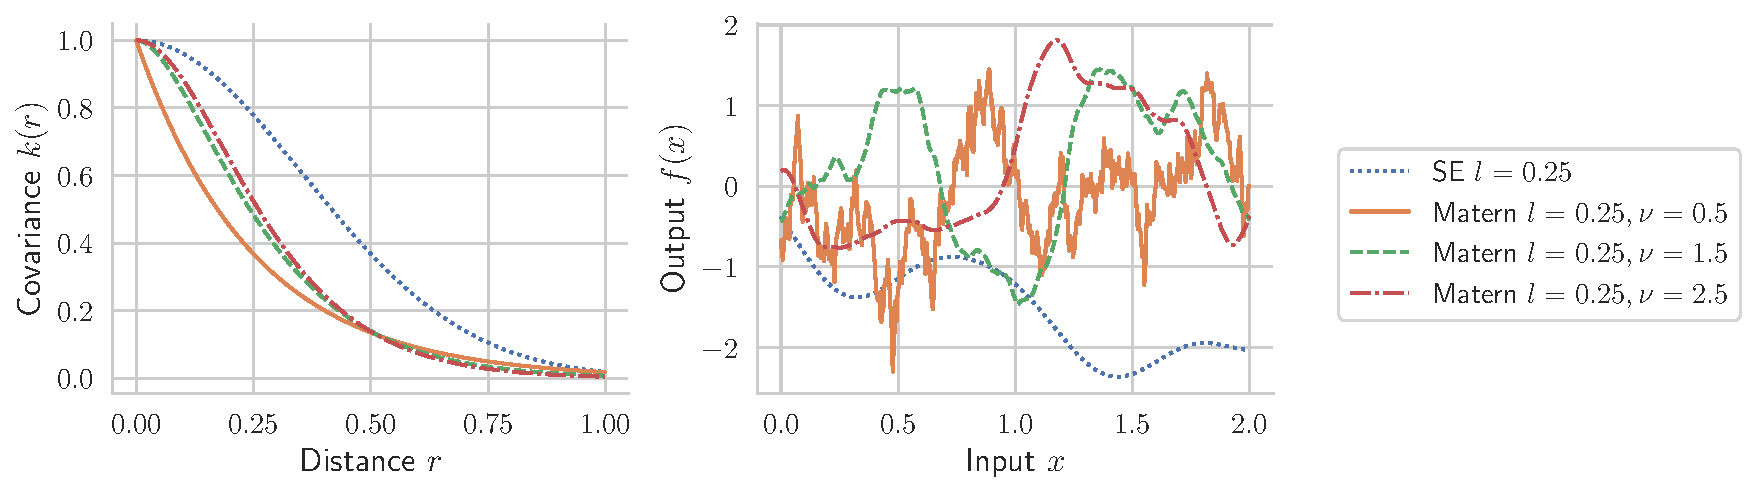
\includegraphics[width=\textwidth]{res/covariance_overview.pdf}
    \caption{Overview of different kernel functions. SE is squared exponential, $l$ is lengthscale, $\nu$ is the smoothness parameter. \textbf{Left}: covariance functions as function of distance. \textbf{Right}: one prior function $f \sim \mathcal N(\vect 0, K_{XX})$ sampled for each kernel.}
    \label{fig:kernel_overview}
\end{figure}

\begin{comment}
\begin{figure}
    \centering
    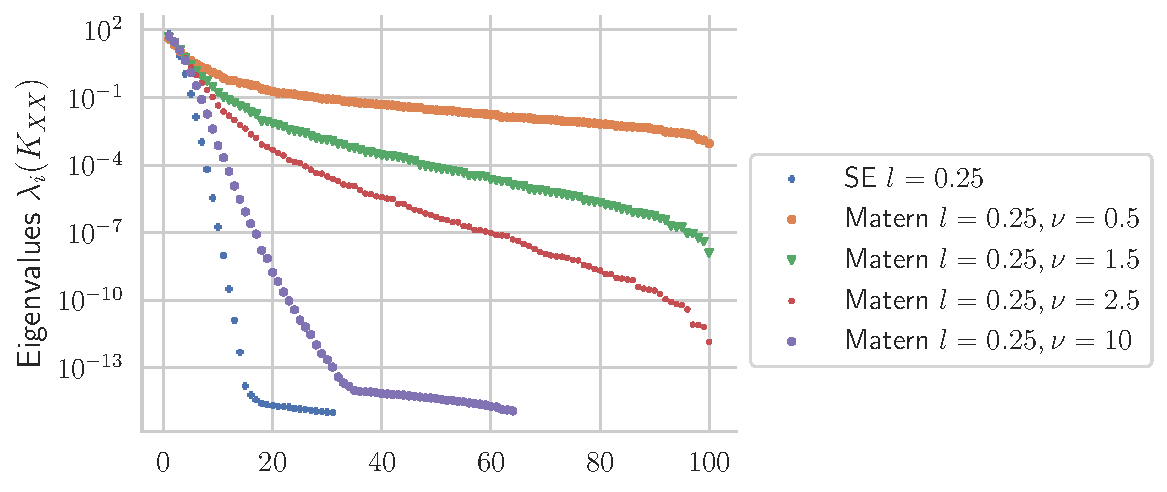
\includegraphics[width=0.6\textwidth]{res/kernel_eigenvalues.pdf}
    \caption{Eigenvalues of the kernel matrix $K_{XX}$ on a random grid $x_1, \ldots, x_{100} \sim \mathcal U([0, 1])$. Noise variance was set to $\sigma^2 = 0.1$.
    %Eigenvalues of the kernel matrix $K_{XX}$ on a uniform grid $x_i \in [0, 1], \, i = 1, \ldots, 100$. Eigenvalues below $10^{-15}$ were set to exactly zero.
    }
    \label{fig:kernel_mx_eigvals}
\end{figure}
\end{comment}

\begin{figure}
    \centering
    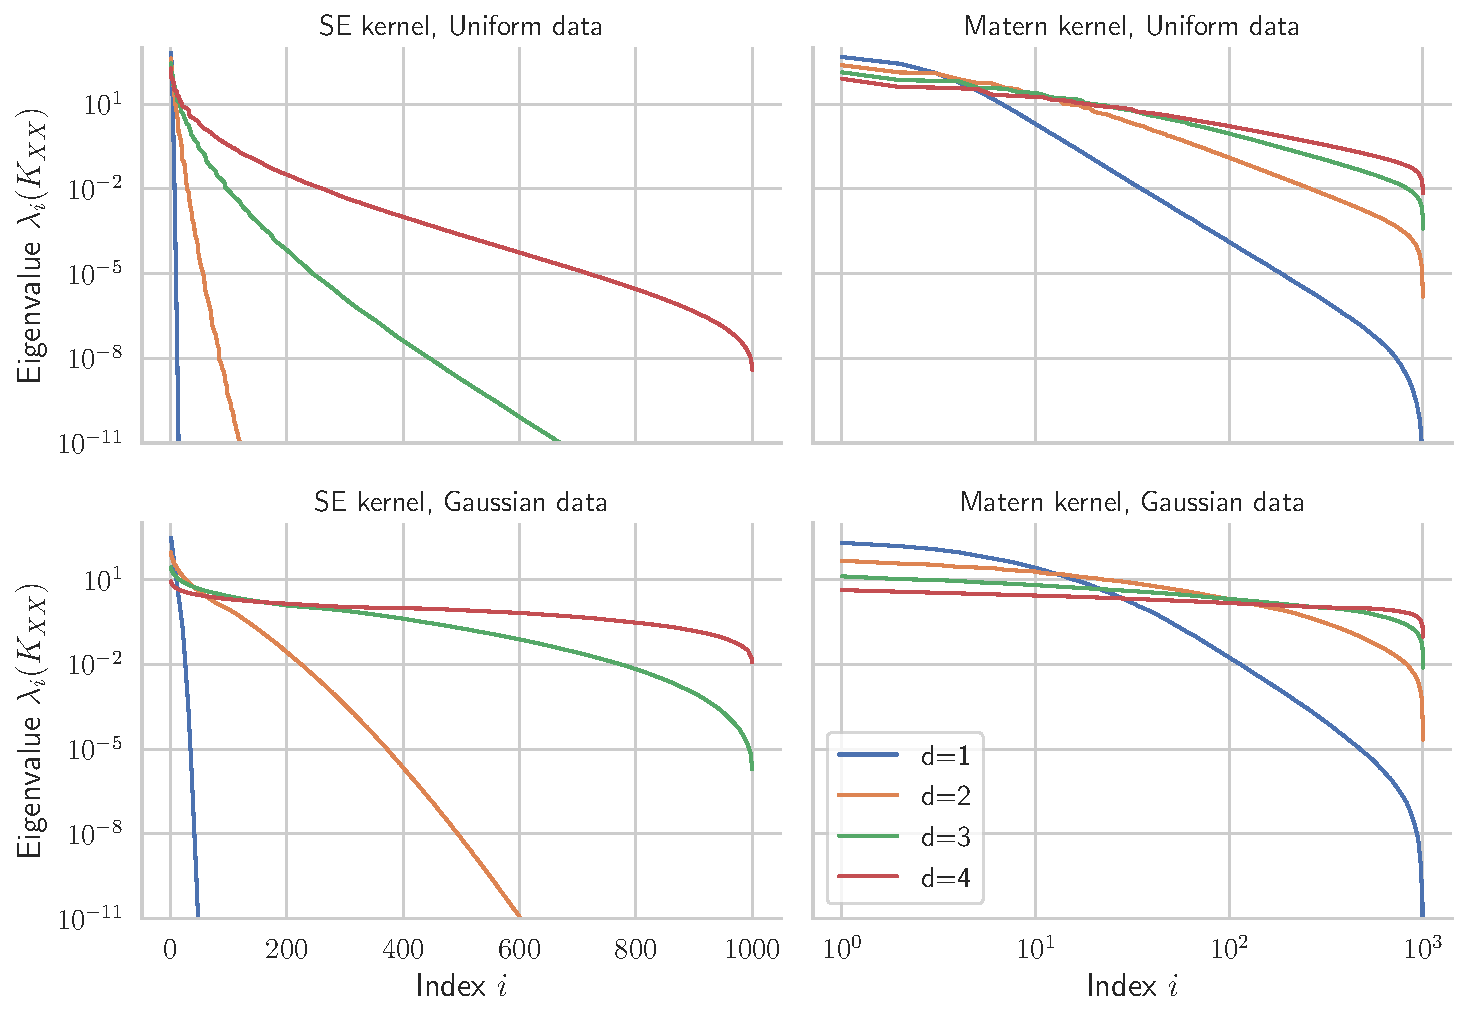
\includegraphics[width=0.75\textwidth]{report/res/kernel_eigvals.pdf}
    \caption{Eigenvalues of the kernel matrix on $1000$ data points $\vect x_i \sim \mathcal D$ for different distribution $\mathcal D$ in dimension $d=1,2,3,4$. Values shown are averaged over 5 runs. \textbf{Upper row}: Uniform data $\mathcal D = \mathcal U([0,1]^d)$, \textbf{bottom row}: Gaussian data  $\mathcal D = \mathcal N(\vect 0_d, \mathbb I_d)$. \textbf{Left column}: squared exponential kernel with lengthscale $l = 0.25$, \textbf{right column}: Matern kernel with lengthscale $l=0.25$ and smoothness $\nu = 1.5$. 
    %Effect of the input space dimension on the spectral decay of the kernel matrix. The grids are $\vect x_1, \ldots, \vect x_{100} \sim \mathcal U([0, 1]^d)$, noise variance $\sigma^2 = 0.1$. \textbf{Left}: squared exponential kernel with lengthscale $l=0.5$. \textbf{Right}: Matern kernel with $l=0.5, \nu = 2.5$.
    }
    \label{fig:kernel_mx_eigvals}
\end{figure}

\subsection{Pivoted Cholesky on Kernel Matrices}

We use $1000$ data points $\vect x_i \sim \mathcal D$ for the uniform and Gaussian distribution in several dimensions with the SE and Matern kernels. We run up to $k_{\max} = 300$ steps of pivoted Cholesky, early stopping whenever $\trace(E_k)$ drops below the tolerance $10^{-10}$. 

The growth factor $\Gamma_k$ of Theorem~\ref{thm:pivchol_decay} is shown in Figure~\ref{fig:pivchol_gamma}. Recall that the theoretical worst case is $\Gamma_k = \mathcal O(4^k)$. For the kernel matrices we consider here, we have linear growth at worst. 
Comparing the balance between spectral decay and the growth of the gamma factor, we show in Figure~\ref{fig:pivchol_upperbound} the factor $\Gamma_k \lambda_k(K_{XX})$ appearing in the upper bound of $\trace(E_k)$ in Theorem~\ref{thm:pivchol_decay}. For the cases with slow spectral decay (see Figure~\ref{fig:kernel_mx_eigvals}), the upper bound might not even decay with the rank $k$, giving no guarantees on the efficiency of pivoted Cholesky as a preconditioner. 
Eventually, the condition number of the kernel matrix preconditioned with pivoted Cholesky in Figure~\ref{fig:pivchol_cond}. For Gaussian data in dimension $d> 1$, the preconditioner has little effect, but the matrices are well conditioned in the first place.

\begin{figure}
    \centering
    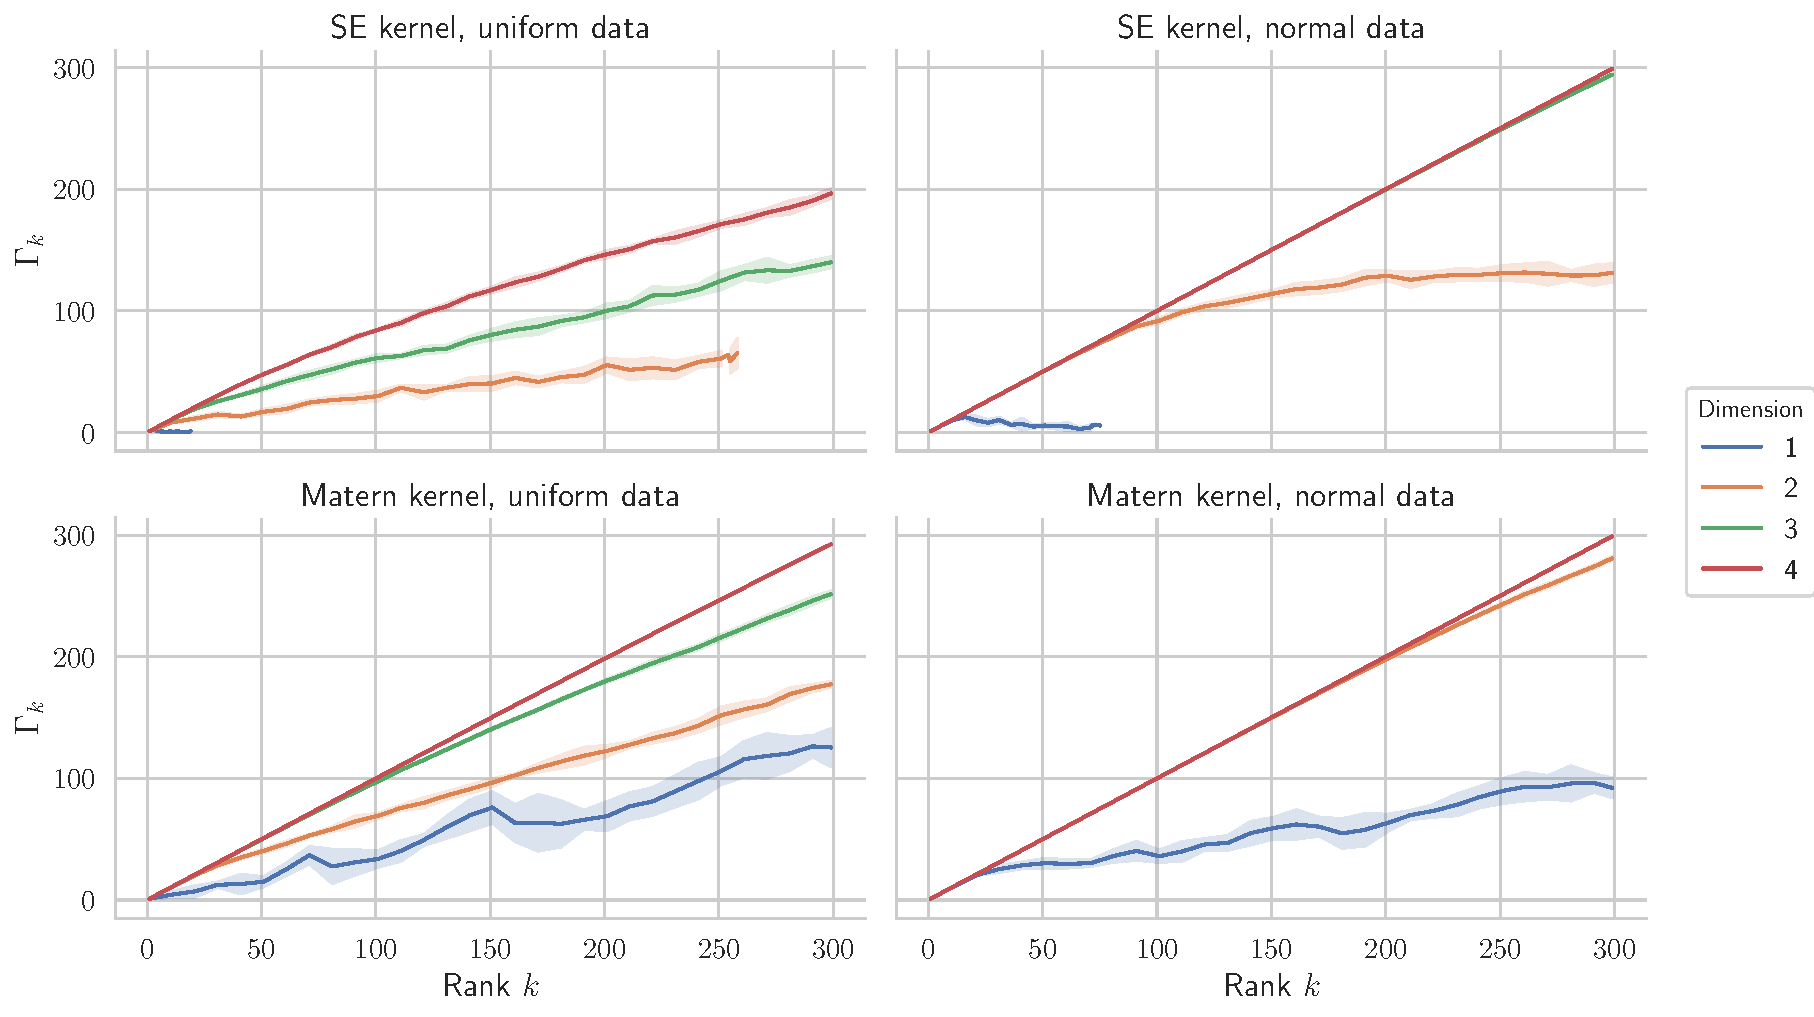
\includegraphics[width=0.85\textwidth]{report/res/pivchol_gamma.pdf}
    \caption{Factor $\Gamma_k$ of Theorem~\ref{thm:pivchol_decay} for pivoted Cholesky run on $K_{XX}$ with $1000$ data points $\vect x_i \sim \mathcal D$. Values are averaged over five runs, shaded areas represent $\pm$ standard deviation. \textbf{Columns}: uniform (left) and Gaussian (right) data. \textbf{Rows}: squared exponential (top) and Matern (bottom) kernels. }
    \label{fig:pivchol_gamma}
\end{figure}

\begin{figure}
    \centering
    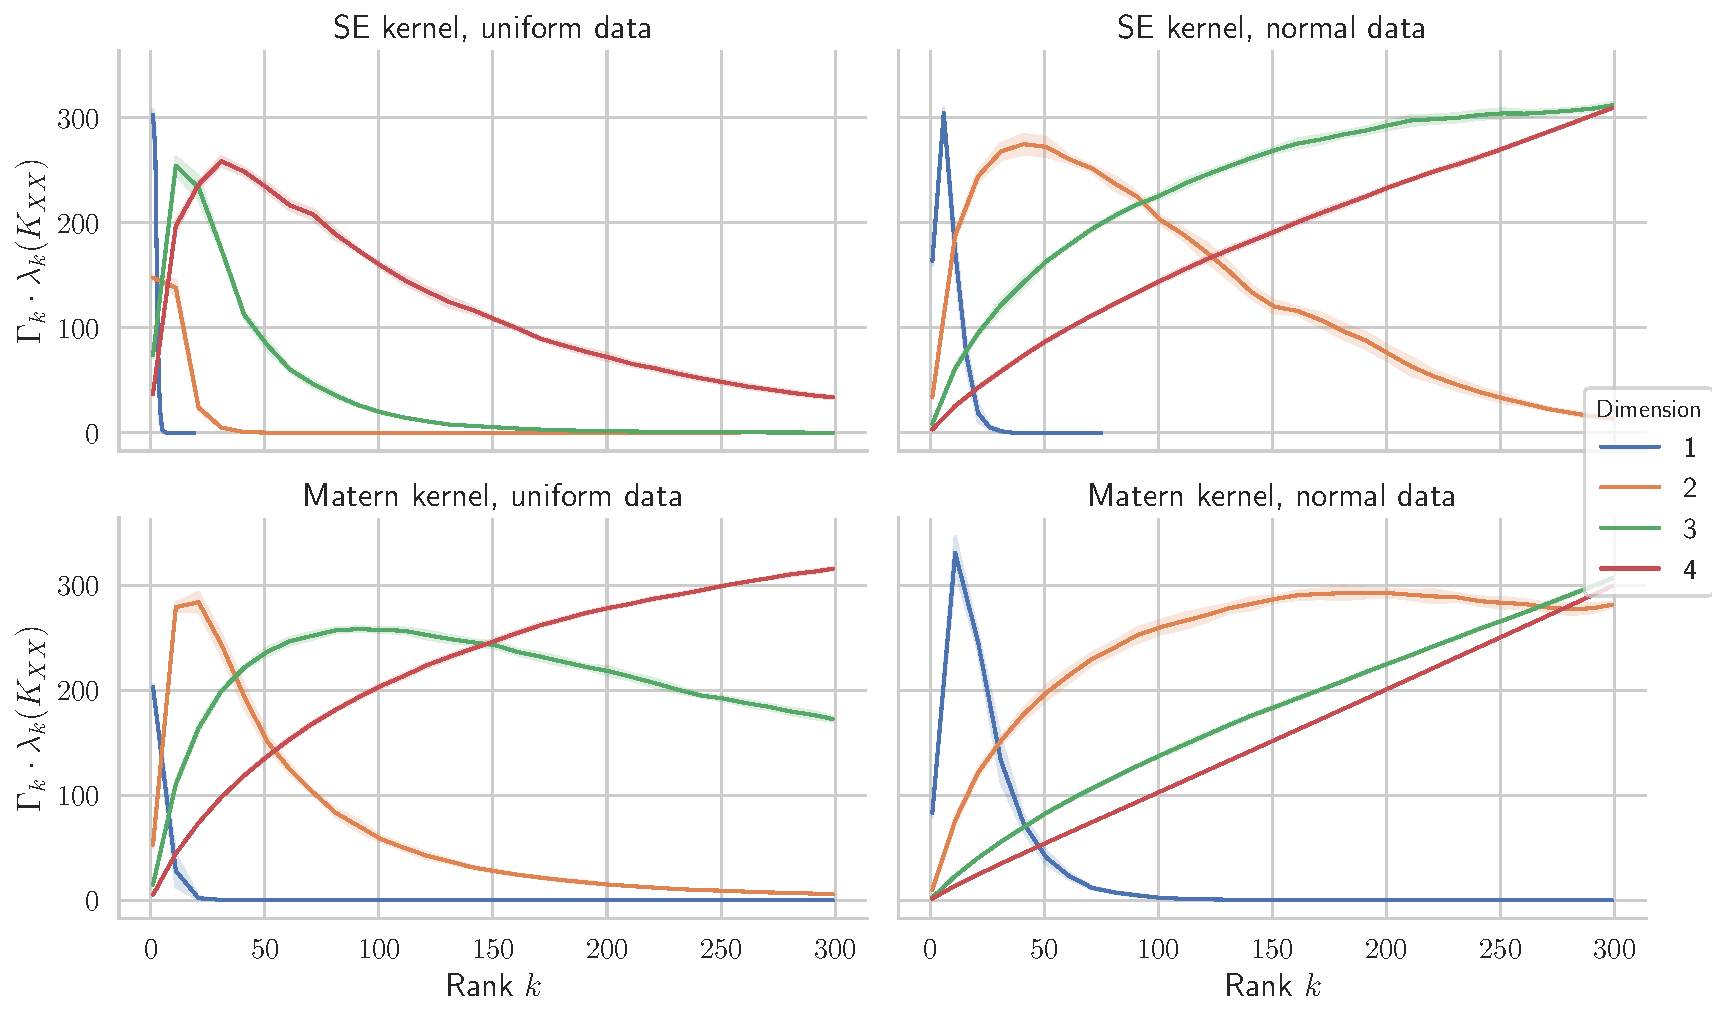
\includegraphics[width=0.85\textwidth]{report/res/pivchol_upperbound.pdf}
    \caption{Upperbound $\Gamma_k \lambda_k(K_{XX})$ of Theorem~\ref{thm:pivchol_decay} for pivoted Cholesky run on $K_{XX}$ with $1000$ data points $\vect x_i \sim \mathcal D$. Values are averaged over five runs, shaded areas represent $\pm$ standard deviation. \textbf{Columns}: uniform (left) and Gaussian (right) data. \textbf{Rows}: squared exponential (top) and Matern (bottom) kernels. }
    \label{fig:pivchol_upperbound}
\end{figure}

\begin{figure}
    \centering
    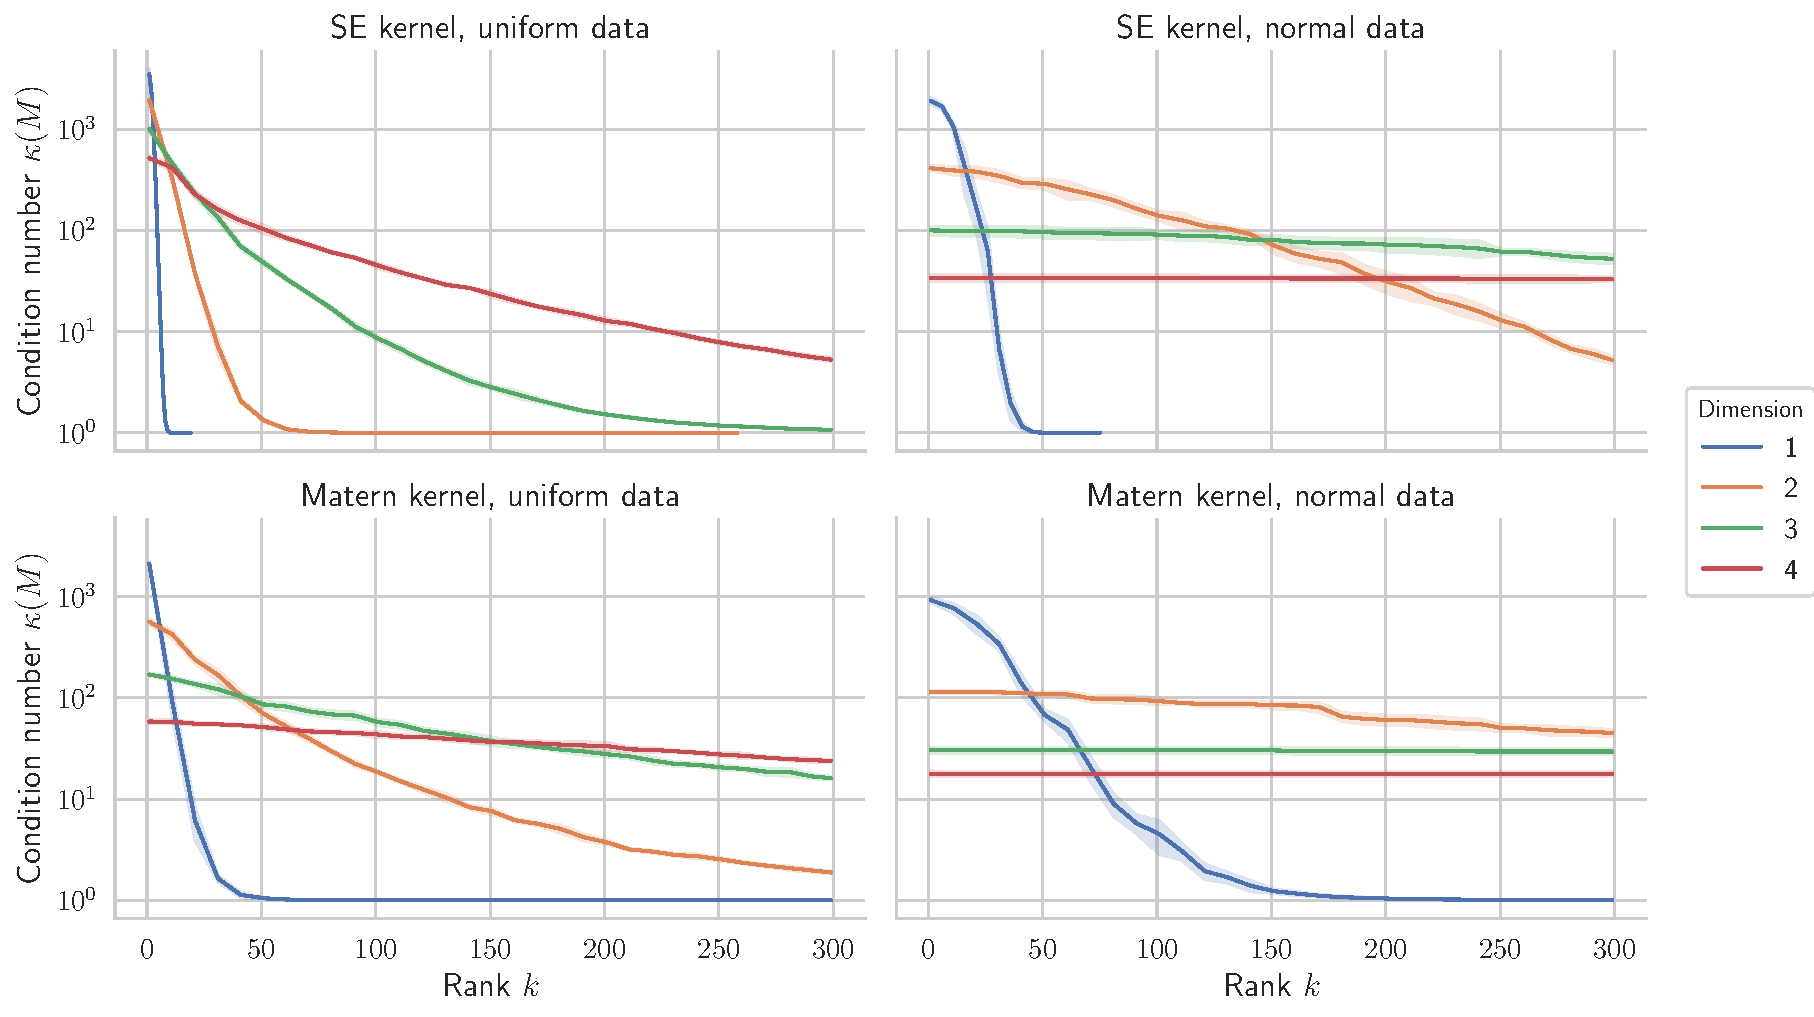
\includegraphics[width=0.85\textwidth]{report/res/pivchol_cond.pdf}
    \caption{Condition number of the preconditioned matrix $M := \widehat P^{-1/2}_k \widehat K_{XX} \widehat P^{-1/2}_k$ with $1000$ data points $\vect x_i \sim \mathcal D$. Values are averaged over five runs, shaded areas represent $\pm$ standard deviation. \textbf{Columns}: uniform (left) and Gaussian (right) data. \textbf{Rows}: squared exponential (top) and Matern (bottom) kernels. }
    \label{fig:pivchol_cond}
\end{figure}




\subsection{Lanczos quadrature and Log Determinant Estimation}

We compare the bounds of Theorem \ref{thm:cortinovis} for Lanczos tridiagonalizations computed with mBCG. We use custom matrices to have control on the spectra. 
Recall for a fixed relative error $\epsilon$, the estimated number of probe vectors $N$ is mainly driven by the ratio $r = \norm{\log A}_F^2 / \trace(\log A)^2$. 
In Figure~\ref{fig:logdet_mbcg}, we compare log-det estimation for a matrix with ratio $r \ll 1$ (left panel) and with $r \approx 1$ (right panel).
The case $r \ll 1$ requires very few probe vectors and iterations, as the variance of the estimator and the error of Lanczos are small compared to the trace. The case $r \approx 1$ compares unfavorably to using $n$ probe vectors with the canonical basis. 

We show the error of Lanczos quadrature with preconditioning for an example kernel matrix in Figure~\ref{fig:quadrature}. 
Each curve represents a different rank $k$ of the preconditioner, and hence represent estimation of quadratures with different matrices. Comparing the slopes shows preconditioning allows to decrease the number of iterations. 

\begin{figure}
    \centering
    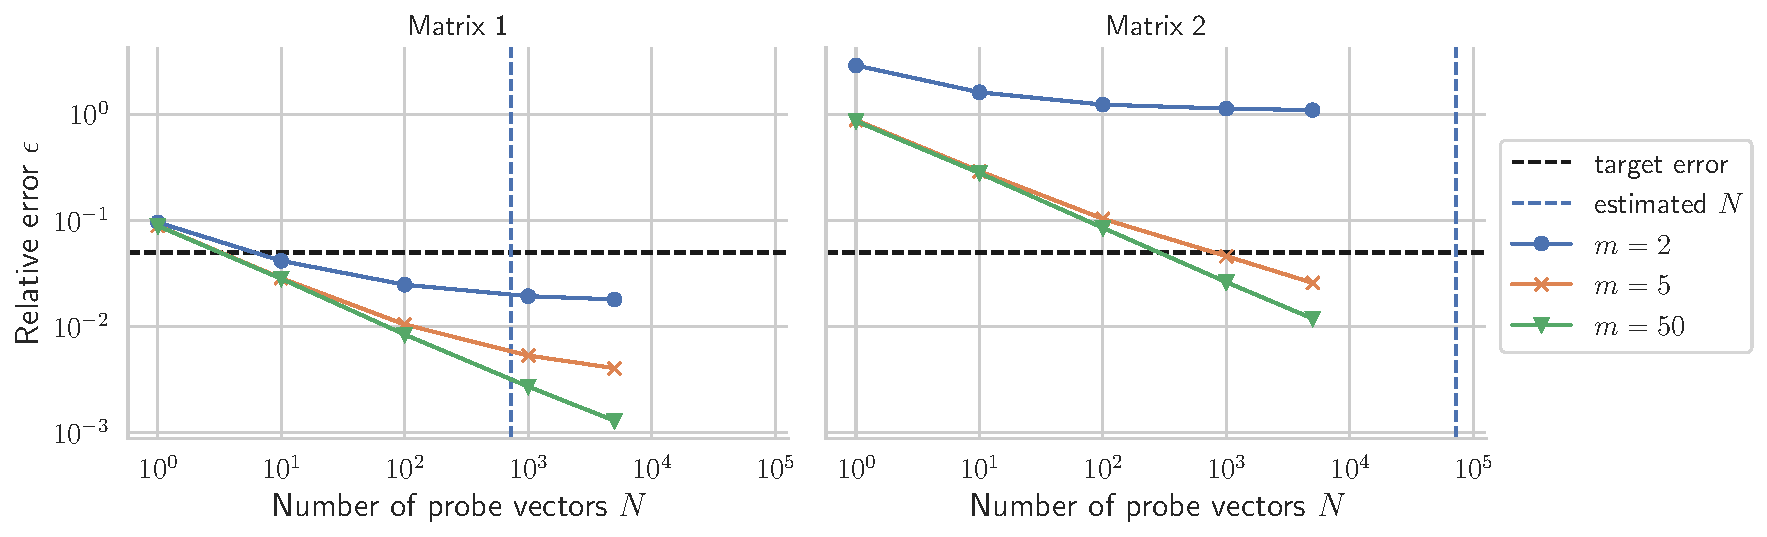
\includegraphics[width=\textwidth]{res/logdet_mbcg.pdf}
    \caption{Log determinant estimation with stochastic Lanczos quadrature where partial tridiagonal matrices were computed with mBCG algorithm, no preconditioning used. The matrices are $A = Q \Lambda Q^\top \in \R^{n \times n}$ with $n=1000$, $Q$ orthogonal and $\Lambda = \text{diag}(\lambda_1, \ldots, \lambda_n)$. The $95^\text{th}$ error quantiles are plotted. \textbf{Left}: $\lambda_i = i, \, 1 \le i \le n$, the estimated $m$ value is 51. \textbf{Right}: $\lambda_i = 10i, \, 1 \le i \le 10$, $\lambda_i = 1, \, 10 < i \le n$, so that $\text{rank}(\log K_{XX}) = 10$. The estimated $m$ value is $132$.}
    \label{fig:logdet_mbcg}
\end{figure}


\begin{figure}
    \centering
    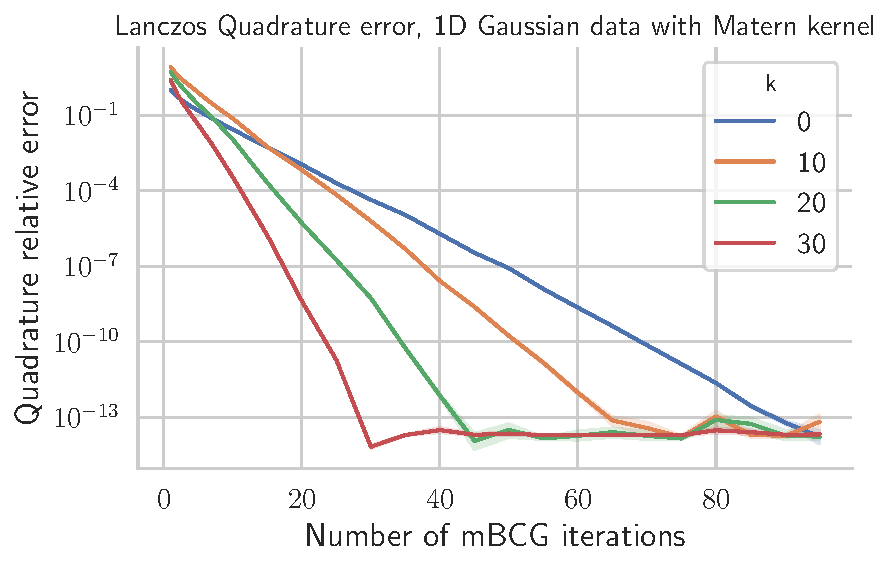
\includegraphics[width=0.5\textwidth]{report/res/quadrature_1d_gaussian_matern.pdf}
    \caption{Error of Lanczos quadrature for the estimate $\norm{\vect z}_2^2 \vect e_1^\top \log(T_m) \vect e_1 \approx \vect z^\top \log(M) \vect e_1$, with $T_m$ the tridiagonalization of the preconditioned matrix $M = \widehat P_k^{-1/2} \widehat K_{XX} \widehat P_k^{-1/2}$ for $k > 0$ and $M = K_{XX}$ for $k=0$. We used 1D Gaussian data with a Matern kernel ($\sigma^2 = 0.1$, $\ell = 0.1$).}
    \label{fig:quadrature}
\end{figure}


\subsection{Computation of Likelihood}

We test computation of likelihood on 2D uniform data with SE kernel. We run as many steps as required for mBCG to reach tolerance $10^{-10}$, as shown in Figure~\ref{fig:likelihood_mbcg_steps}. For a fixed preconditioner rank $k$, the logdet error achieves a Monte Carlo rate $\mathcal O(N^{-1/2})$ in Figure~\ref{fig:likelihood_logdet}, whereas increasing $k$ makes the preconditioner capture most of the logdet (see Equation~\ref{eq:logdet_precond}). The error on the trace term is independent of $k$ and achieves a Monte Carlo rate as well, see Figure~\ref{fig:likelihood_traces}. The final errors on the likelihood and the gradient (Equations~\ref{eq:marginal_log_likelihood}, \ref{eq:marginal_log_likelihood_gradient}) are shown in Figures~\ref{fig:likelihood_likelihood}, \ref{fig:likelihood_grad}.


\begin{figure}
    \centering
    \subfigure[]{\label{fig:likelihood_mbcg_steps}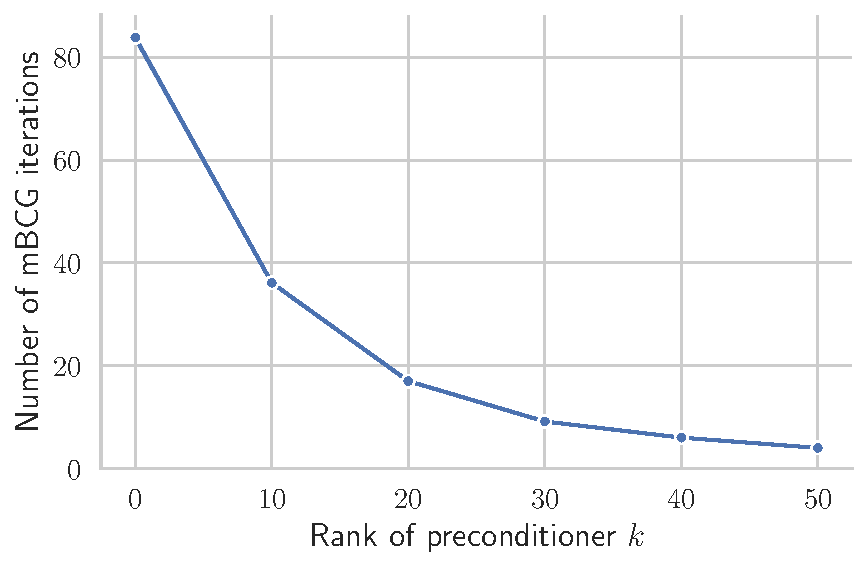
\includegraphics[width=0.3\textwidth]{report/res/likelihood_mbcg_steps.pdf}}
    \subfigure[]{\label{fig:likelihood_logdet}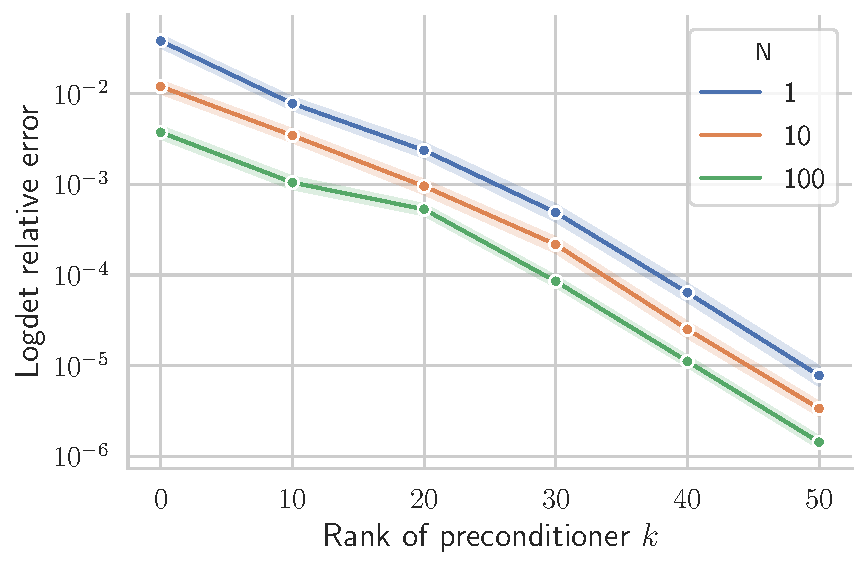
\includegraphics[width=0.3\textwidth]{report/res/likelihood_logdet.pdf}}
    \subfigure[]{\label{fig:likelihood_traces}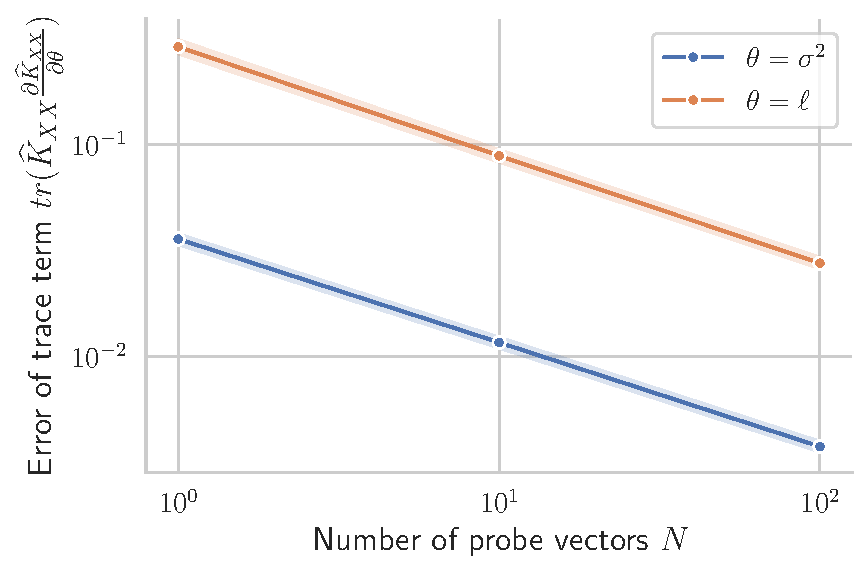
\includegraphics[width=0.3\textwidth]{report/res/likelihood_traces.pdf}}
    \subfigure[]{\label{fig:likelihood_likelihood}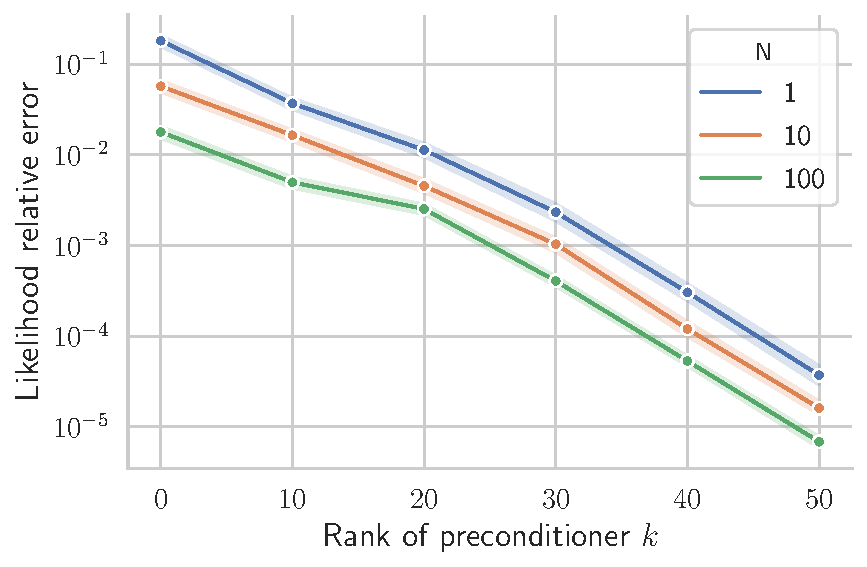
\includegraphics[width=0.3\textwidth]{report/res/likelihood_likelihood.pdf}}
    \subfigure[]{\label{fig:likelihood_grad}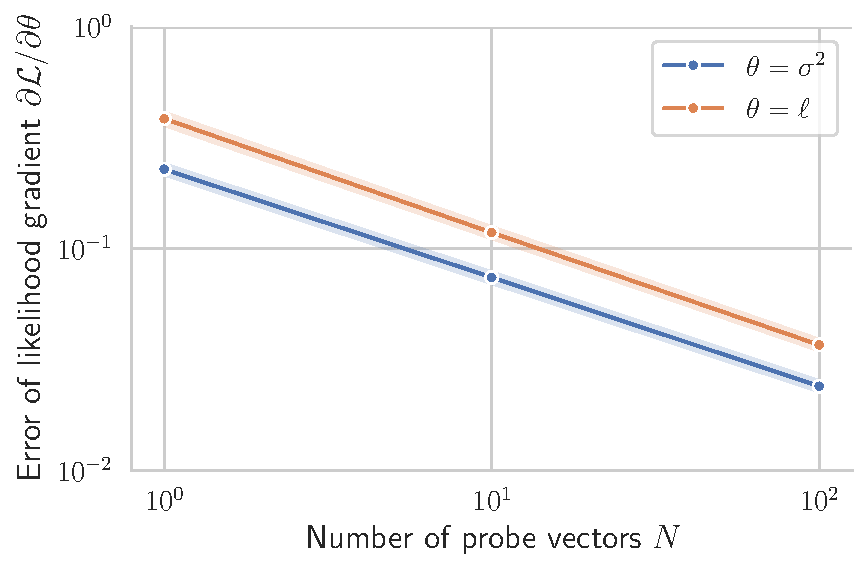
\includegraphics[width=0.3\textwidth]{report/res/likelihood_gradient.pdf}}
    \label{fig:likelihood}
    \caption{Likelihood computation for 2D uniform data with SE kernel ($\sigma^2 = 0.1, \ell = 0.2$).}
\end{figure}


% -----------------------------------------------------


\begin{comment}
\subsection{Logdet Estimation of Kernel Matrix with Preconditioning}

\begin{figure}
    \centering
    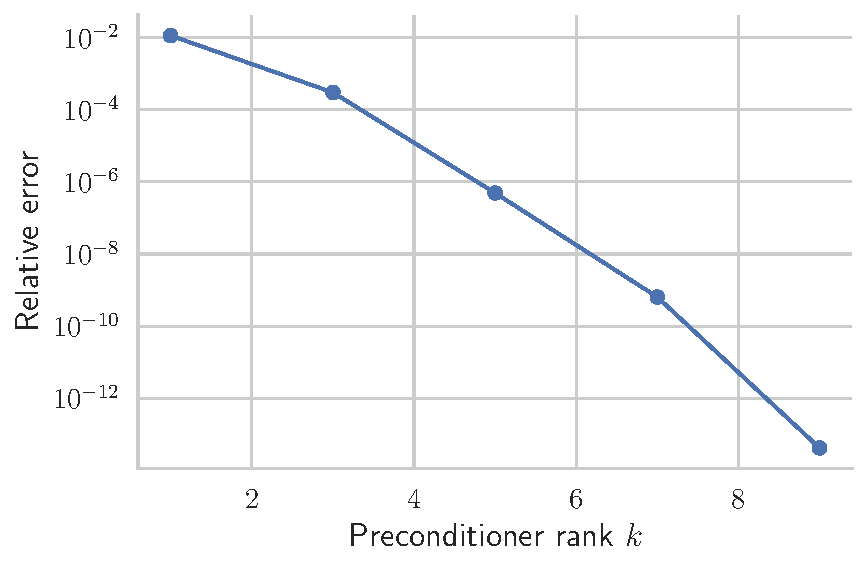
\includegraphics[width=0.5\textwidth]{res/logdet_precond_errvsk.pdf}
    \caption{Log determinant estimation of Kernel matrix with preconditioning. The kernel matrix is the SE kernel on the uniform grid $x_1, \ldots, x_n \in [0, 1], \, n=100$. The logdet is $\log\det \widehat K_{XX} = \log\det \widehat P_k + \log\det(\widehat P^{-1} \widehat K_{XX})$ where the logdet of the preconditioned matrix is computed with stochastic Lanczos quadrature. $N=100$ probe vectors are used and $m$ is large enough to reach tolerance $10^{-10}$.}
    \label{fig:my_label}
\end{figure}


\begin{figure}
    \centering
    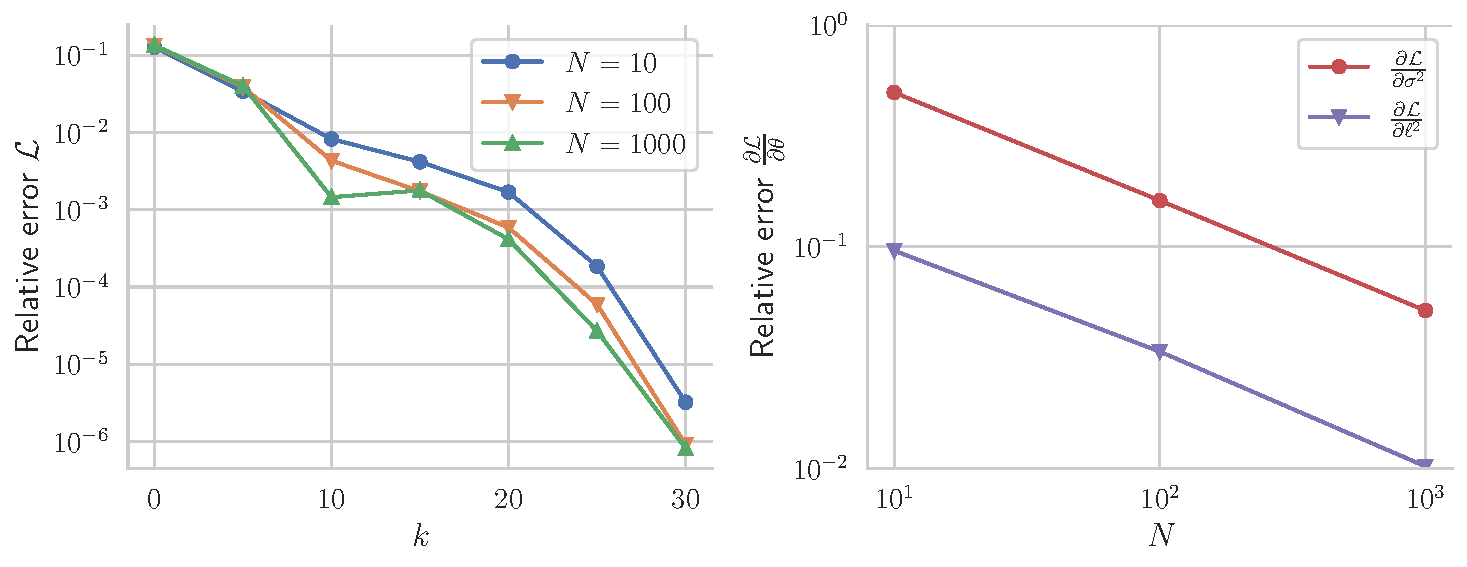
\includegraphics[width=0.9\textwidth]{report/res/likelihood.pdf}
    \caption{Average error and timing benchmark of the marginal log likelihood ($\mathcal L$) computed from mBCG output with pivoted Cholesky preconditioning over 10 runs. The data is $x_1, \ldots, x_{1000} \sim \mathcal U([0, 1]), \, y_i = \sin(2\pi x_i)$. mBCG steps $m$ was left unspecified to reach tolerance $10^{-10}$. Kernel parameters: $l = 0.25, \, \nu = 2.5$.}
    \label{fig:likelihood}
\end{figure}

\begin{figure}
    \centering
    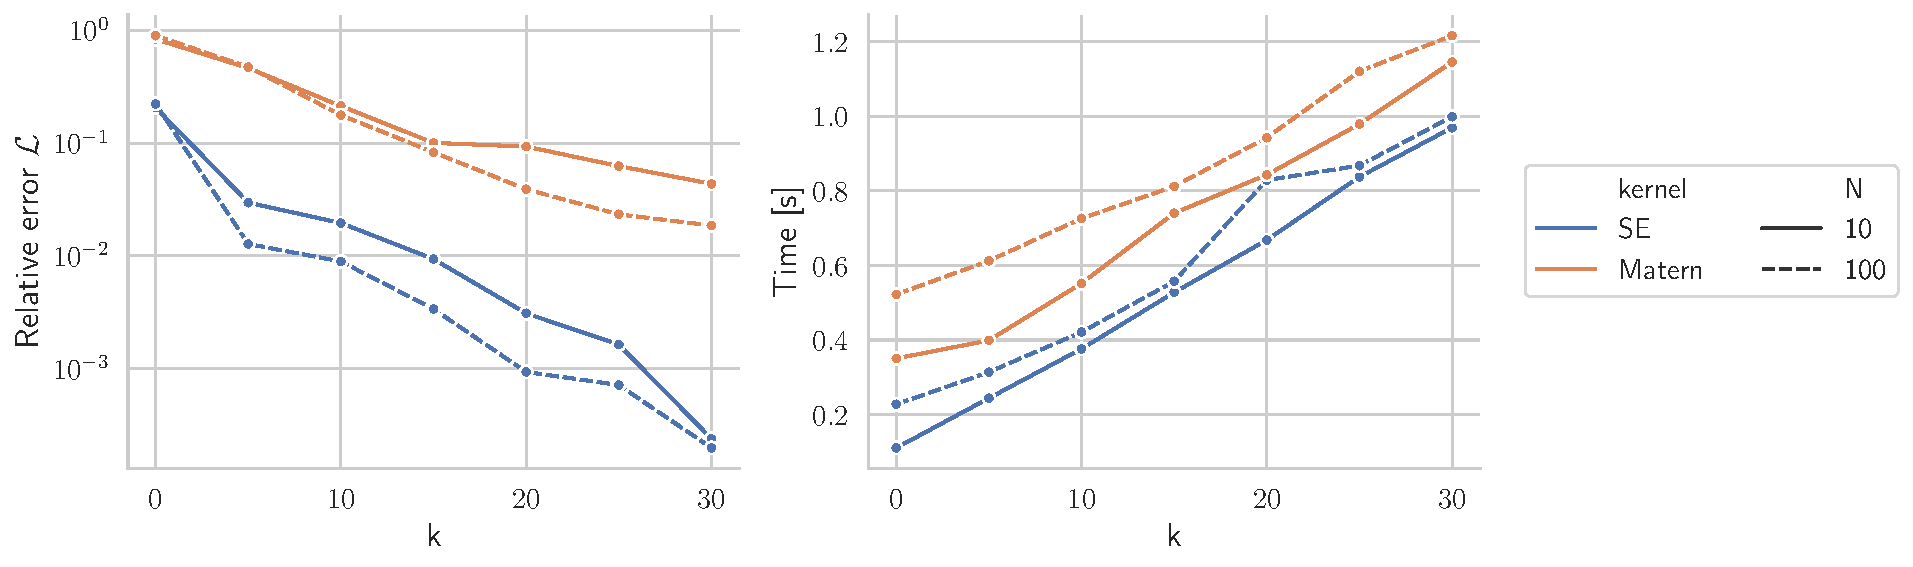
\includegraphics[width=0.9\textwidth]{report/res/likelihood_2d_unif.pdf}
    \caption{Same as Figure \ref{fig:likelihood} but with data $\sim \mathcal U([0,1]^2)$.}
    \label{fig:likelihood_2d_unif}
\end{figure}

\begin{figure}
    \centering
    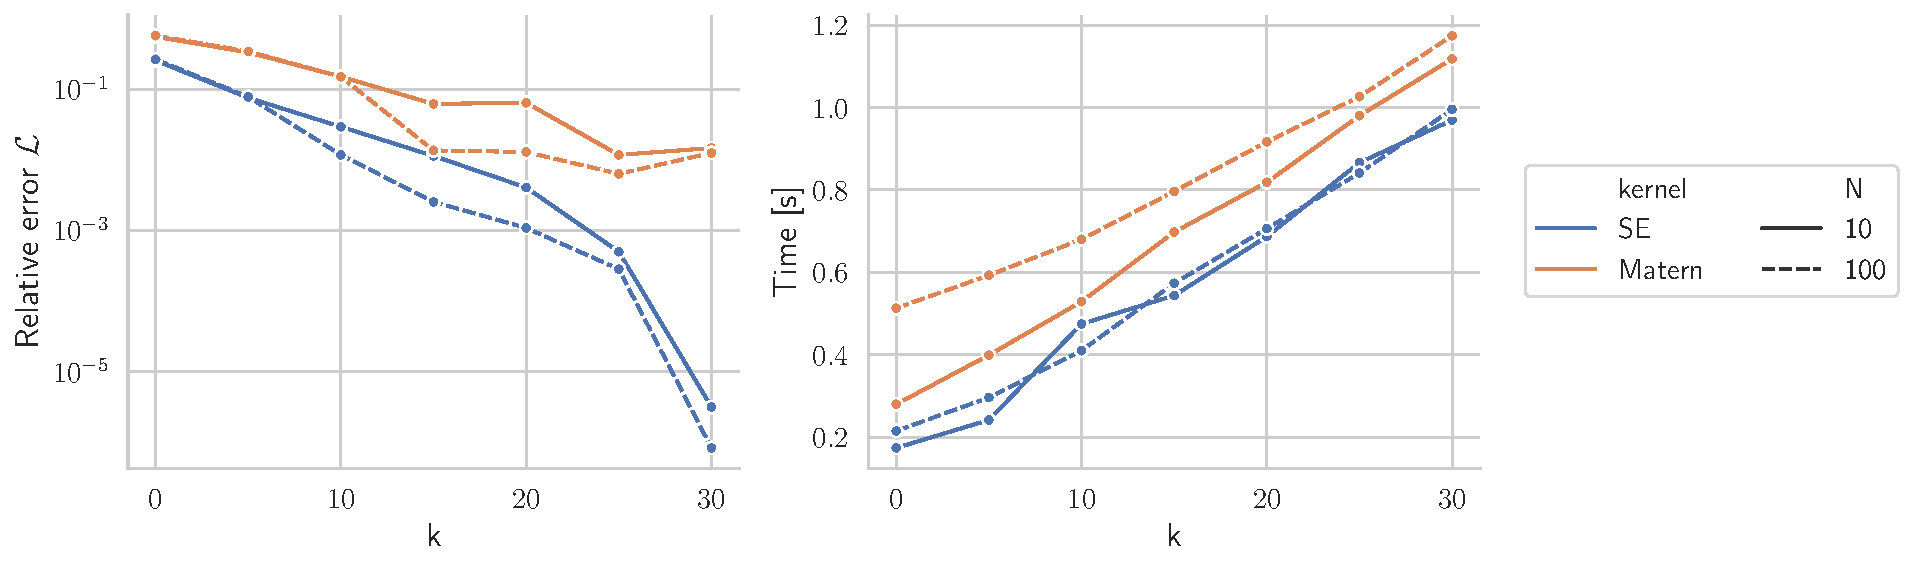
\includegraphics[width=0.9\textwidth]{report/res/likelihood_1d_stdnormal.pdf}
    \caption{Same as Figure \ref{fig:likelihood} but with data $\sim \mathcal N(0, 1)$.}
    \label{fig:likelihood_1d_stdnormal}
\end{figure}
\end{comment}



% ----------------------------------------------


\newpage
\printbibliography


% ----------------------------------------------
\newpage
\appendix
\appendixpage

\section{Appendix - Gradient of Marginal Log-Likelihood} \label{sec:marginal_log_likelihood_gradient}

Starting from the marginal log-likelihood \eqref{eq:marginal_log_likelihood}, we wish to calculate the expression of its gradient with respect to hyperparameters $\theta_i$. We first compute the derivative of the inverse of a matrix using the chain rule,

\begin{equation*}
    \mymathbb 0 = \frac{d}{d \theta} \Id = \frac{d}{d \theta} \left( A^{-1}(\theta) A(\theta) \right) = \frac{d A^{-1}(\theta)}{d \theta} A(\theta) + A^{-1}(\theta) \frac{d A(\theta)}{d \theta}
     \;,
\end{equation*}

which yields

\begin{equation*}
    \frac{d A^{-1}(\theta) }{d \theta} = - A^{-1}(\theta) \frac{d A(\theta)}{d \theta} A^{-1}(\theta) \; .
\end{equation*}


The derivative of the determinant can be obtained with the Jacobi's formula %\textbf{TODO should I prove it? quite beautiful proof! recall NIDS lecture for polynomial invariants of deg > 3}
,

\begin{equation*}
    \frac{d}{d \theta} \det A(\theta) = \det (A(\theta)) \cdot \trace \left( A^{-1}(\theta) \frac{d A(\theta)}{d \theta} \right) \; .
\end{equation*}

Applying it on the log determinant will cancel the $\det A(\theta)$ term. We retrieve Equation \eqref{eq:marginal_log_likelihood_gradient} by substitution of the above quantities for $A(\theta) := \widehat K_{XX}$ where the dependence of the kernel on hyperparameters is left implicit for notation simplicity.


\section{Appendix --- Algorithms}

We first recall the Lanczos algorithm for linear systems and the preconditioned conjugate gradients algorithm. This introduces notation and serves as a reference for the derivation of Lanczos from CG as described in section \ref{sec:lanczos_from_cg}. We then present the mBCG algorithm, which combines Lanczos and CG extended to multiple right-hand sides, the reader can then spot differences with vanilla CG. We also provide a detailed explanation of batched computations for mBCG, both in terms of mathematical notation and programmatic implementation. 


\vspace{0.5cm}

\begin{algorithm}[H]
 \label{algo:lanczos}
\SetAlgoLined
\SetKwInOut{Input}{Input}
\SetKwInOut{Output}{Output}
\DontPrintSemicolon
\Input{matrix-vector multiplication oracles $\vect a \mapsto \widehat K_{XX} \vect a$, right-hand side $\vect b$, starting vector $\vect u_0$, number of steps $m$}
\Output{approximate solution $\vect u_m \approx \widehat K_{XX}^{-1} \vect b$, orthonormal basis $V_m$, tridigonal matrix $T_m$}
 %\tcp{Initialize residuals}
 $\vect r_0 \leftarrow \vect b - \widehat K_{XX} \vect x_0, \; \beta \leftarrow \norm{\vect r_0}_2$ \;
 %\tcp{Initialize basis for Krylov subspace}
 $\vect v_1 \leftarrow \vect r_0 / \beta$ \;
 \For{$k = 1, \ldots, m$}{
    $\tilde{\vect w} \leftarrow \widehat K_{XX} \vect v_k - \eta_k \vect v_{k-1}$ \tcp*{if k=1, set $\eta_1 \vect v_0 := \vect 0$}
    $\delta_k \leftarrow \vect v_k^\top \tilde{\vect w}$ \;
    $\vect w_k \leftarrow \tilde{\vect w} - \delta_k \vect v_k$ \;
    $\eta_k \leftarrow \norm{\vect w_k}_2$ \;
    $\vect v_{k+1} \leftarrow \vect w_l / \eta_k$ \; 
 }
 $V_m = \begin{bmatrix} \vect v_1 & \dots & \vect v_m \end{bmatrix}, \; T_m = \text{tridiag}(\eta_{k-1}, \delta_k, \eta_k)$ \;
 Compute $\vect y_m = \beta T_m^{-1} \vect e_1$ and $\vect u_m = \vect u_0 + V_m \vect y_m$ \;
 
 \caption{Lanczos algorithm to solve linear system $\widehat K_{XX} \vect u = \vect b$}
\end{algorithm}


\begin{algorithm}[H]
 \label{algo:pcg}
\SetAlgoLined
\SetKwInOut{Input}{Input}
\SetKwInOut{Output}{Output}
\DontPrintSemicolon
\Input{matrix-vector multiplication oracles $\vect a \mapsto \widehat K_{XX} \vect a$ and $\vect a \mapsto P^{-1} \vect a$, right-hand side $\vect b$, number of steps $m$}
\Output{approximate solution $\vect u_m \approx \widehat K_{XX}^{-1} \vect b$}
 \tcp{Initialize solution and residuals}
 $\vect u_0 \leftarrow \vect 0, \; \vect r_0 \leftarrow \vect b$ \;
 \tcp{Initialize preconditioned residuals and first search direction}
 $\vect z_0 \leftarrow P^{-1} \vect r_0$ \;
 $\vect d_1 \leftarrow \vect r_0$ \;
 
 \For{$k = 1, \ldots, m$}{
    \tcp{Line search: optimal step size in direction $\vect d_k$}
    $\alpha_k \leftarrow \vect r_k^\top \vect z_k \,/\, \vect d_k^\top (\widehat K_{XX} \vect d_k)$ \;
    \tcp{Update solution and residuals}
    $\vect u_k \leftarrow \vect u_{k-1} + \alpha_k \vect d_k$ \;
    $\vect r_k \leftarrow \vect r_{k-1} - \alpha_k \widehat K_{XX} \vect d_k$ \;
    $\vect z_k \leftarrow P^{-1} \vect r_k$ \;
    \tcp{Conjugate Gram Schmidt and compute next search direction}
    $\beta_k \leftarrow \vect r_k^\top \vect z_k \,/\, \vect r_{k-1}^\top \vect z_{k-1}$ \;
    $\vect d_{k+1} \leftarrow \vect z_k + \beta_k \vect d_k$ \;
 }
 \caption{Vanilla conjugate gradients to solve $\widehat K_{XX} \vect u = \vect b$}
\end{algorithm}

\vspace{0.5cm}

\begin{algorithm}[H]
 \label{algo:mBCG}
\SetAlgoLined
\SetKwInOut{Input}{Input}
\SetKwInOut{Output}{Output}
\DontPrintSemicolon
\Input{matrix-matrix multiplication oracles $A \mapsto \widehat K_{XX} A$ and $A \mapsto P^{-1} A$, right-hand side $B = \begin{bmatrix}
\vect y & \vect z_1 & \ldots & \vect z_N
\end{bmatrix}$, number of steps $m$}
\Output{approximate solutions $U_m \approx \widehat K_{XX}^{-1} B$, partial Lanczos tridiagonalizations $T_m^{(i)}$}
 \tcp{Initialize solutions and residuals}
 $U_0 \leftarrow \mymathbb 0_{n \times (N+1)}$ \;
 $R_0 \leftarrow B$ \;
 \tcp{Initialize preconditioned residuals and search directions}
 $Z_0 \leftarrow P^{-1} R_0$ \;
 $D_1 \leftarrow R_0$ \;
 \tcp{Initialize tridigonal matrices}
 $T_m^{(1)}, \ldots, T_m^{(N)} \leftarrow \mymathbb 0_{m \times m}$ \;
 \For{$k = 1, \ldots, m$}{
    \tcp{Line search: optimal step sizes in directions $D_k$}
    $\vect \alpha_k \leftarrow \varphi(R_k, Z_k) \, ./ \, \varphi(D_k, \widehat K_{XX} D_k)$ \;
    \tcp{Update solutions and residuals}
    $U_k \leftarrow U_{k-1} + D_k \, \text{diag}(\vect\alpha_k)$ \; % (\vect 1 \vect\alpha_k^\top) \odot D_k
    $R_k \leftarrow R_{k-1} - \widehat K_{XX} D_k \, \text{diag}(\vect \alpha_k)$ \; % (\vect 1 \vect\alpha_k^\top) \odot (\widehat K_{XX} D_k)
    $Z_k \leftarrow P^{-1} R_k$ \;
    \tcp{Conjugate Gram Schmidt and compute next search directions}
    $\vect\beta_k \leftarrow \varphi(R_k, Z_k) \,./\, \varphi(R_{k-1}, Z_{k-1})$ \;
    $D_{k+1} \leftarrow Z_{k} + D_k \, \text{diag}(\vect\beta_k)$ \; % (\vect 1 \vect\beta_k^\top) \odot D_k
    \tcp{Compute tridiagonal matrices}
    $[T_m^{(i)}]_{kk} \leftarrow 1 / [\vect \alpha_k]_i + [\vect\beta_{k-1}]_i / [\vect\alpha_{k-1}]_i, \quad i=1, \ldots, N$ \;
    $[T_m^{(i)}]_{k-1, k}, \, [T_m^{(i)}]_{k, k-1} \leftarrow \sqrt{[\vect\beta_{k-1}]_i} / [\vect\alpha_k]_i, \quad i=1, \ldots, N$ \;
 }
 \caption{mBCG to solve Equation \eqref{eq:mbcg_equation}}
\end{algorithm}

\vspace{0.5cm}

We discuss how $p$ right-hand sides can be handled simultaneously. Matrix-vector multiplication $\vect a_i \mapsto \widehat K_{XX} \vect a_i$ is trivially extended to matrix-matrix multiplication $A \mapsto \widehat K_{XX} A$ since

\begin{equation*}
    \widehat K_{XX} A = \widehat K_{XX} \begin{bmatrix}
    \vect a_1 & \dots & \vect a_p
    \end{bmatrix}  = \begin{bmatrix}
    \widehat K_{XX} \vect a_1 & \dots & \widehat K_{XX} \vect a_p
    \end{bmatrix} \; .
\end{equation*}

Vectors $\vect \alpha_k, \vect \beta_k \in \R^{p}$ store the coefficients at each step $k$ for the $p$ right-hand sides. Their computation involves the function $\varphi$ which simply generalizes dot products:

\begin{equation*}
    \varphi: \R^{n \times p} \times \R^{n \times p} \to \R^{p}, \quad
    \varphi(\begin{bmatrix}
    \vect a_1 & \dots & \vect a_p
    \end{bmatrix}, \begin{bmatrix}
    \vect b_1 & \dots & \vect b_p
    \end{bmatrix})
    = \begin{bmatrix}
    \vect a_1^\top \vect b_1 & \dots & \vect a_p^\top \vect b_p
    \end{bmatrix}^\top \; ,
\end{equation*}

which is programatically implemented as element-wise multiplication of $A$ and $B$ and then summing across the first dimension. The $./$ symbol then refers to element-wise division. Finally, note that 

\begin{equation*}
    A \, \text{diag}(\vect\alpha) = \begin{bmatrix} \alpha_1 \vect a_1 & \dots & \alpha_p \vect a_p \end{bmatrix}
\end{equation*}

simply weights columns of $A$ by coefficients in $\vect\alpha$. Explicit computation of the diagonal matrix is straightforward to avoid using Numpy's broadcasting rules\footnote{See \url{https://numpy.org/doc/stable/user/basics.broadcasting.html}}, e.g. \texttt{alpha.T * A}. 

\begin{comment}
Finally, denoting $\odot$ the element-wise multiplication and $\vect 1$ a vector full of ones, the expression

\begin{equation*}
    (\vect 1 \vect \alpha^\top) \odot A 
    = \begin{bmatrix}
    \alpha_1 \vect 1 & \dots & \alpha_p \vect 1
    \end{bmatrix} \odot \begin{bmatrix} \vect a_1 & \dots & \vect a_p \end{bmatrix}
    = \begin{bmatrix} \alpha_1 \vect a_1 & \dots & \alpha_p \vect a_p \end{bmatrix} \; ,
\end{equation*}

results in weighting each column of $A$ by coefficients in $\vect\alpha$. This is straightforward to implement using Numpy's broadcasting rules\footnote{See \url{https://numpy.org/doc/stable/user/basics.broadcasting.html}}, e.g. \texttt{alpha.T * A}. 
\end{comment}


\end{document}
